\documentclass[12pt,a4paper,twoside]{article}
\usepackage{graphicx} % Required for inserting images
\usepackage[
backend=biber,
style=apa
]{biblatex} 
\usepackage{amsmath}
\usepackage{amssymb}
\usepackage{float}
\usepackage{caption}
\usepackage[english]{babel}
\usepackage{breqn}
\usepackage{xcolor}
\usepackage{csquotes}
\usepackage[a4paper, margin=1in]{geometry}
\usepackage{setspace}
\usepackage{graphicx}
\usepackage{hyperref}
\usepackage{booktabs}
\usepackage{siunitx}
\usepackage[toc,page]{appendix}

%%%%%%%%%%%%%% Third level subsection %%%%%%%%%%%%%%%%%%%
\usepackage{titlesec}

\titleclass{\subsubsubsection}{straight}[\subsection]

\newcounter{subsubsubsection}[subsubsection]
\renewcommand\thesubsubsubsection{\thesubsubsection.\arabic{subsubsubsection}}
\renewcommand\theparagraph{\thesubsubsubsection.\arabic{paragraph}} % optional; useful if paragraphs are to be numbered

\titleformat{\subsubsubsection}
  {\normalfont\normalsize\bfseries}{\thesubsubsubsection}{1em}{}
\titlespacing*{\subsubsubsection}
{0pt}{3.25ex plus 1ex minus .2ex}{1.5ex plus .2ex}

\makeatletter
\renewcommand\paragraph{\@startsection{paragraph}{5}{\z@}%
  {3.25ex \@plus1ex \@minus.2ex}%
  {-1em}%
  {\normalfont\normalsize\bfseries}}
\renewcommand\subparagraph{\@startsection{subparagraph}{6}{\parindent}%
  {3.25ex \@plus1ex \@minus .2ex}%
  {-1em}%
  {\normalfont\normalsize\bfseries}}
\def\toclevel@subsubsubsection{4}
\def\toclevel@paragraph{5}
%\def\toclevel@paragraph{6}
\def\toclevel@subparagraph{6}
\def\l@subsubsubsection{\@dottedtocline{4}{7em}{4em}}
\def\l@paragraph{\@dottedtocline{5}{10em}{5em}}
\def\l@subparagraph{\@dottedtocline{6}{14em}{6em}}
\makeatother

\setcounter{secnumdepth}{4}
\setcounter{tocdepth}{4}
%%%%%%%%%%%%%%%%%%%%%%%%%%%%%%%%%%%%%%%%%%%%%%%%%%%%%%%%
% Keywords command
\providecommand{\keywords}[1]
{
  \small	
  \textbf{\textit{Keywords---}} #1
}
%%%%%%%%%%%%%%%%%%%%%%%%%%%%%%%%%%%%%%%%%%%%%%%%%%%%%%%%
% % Add abstract environment to book style
% \newenvironment{abstract}%
% {\cleardoublepage \null \vfill \begin{center}%
% 		\bfseries \abstractname \end{center}}%
% {\vfill\null}
%%%%%%%%%%%%%%%%%%%%%%%%%%%%%%%%%%%%%%%%%%%%%%%%%%%%%%%
% Set font to Times New Roman
%\usepackage{mathptmx}

% Set double spacing
\doublespacing


\addbibresource{bibliography.bib}

\title{Solar and Wind Power Generation Modeling for the Spanish Electrical System}
% \author{Fernando Celaya}
\date{\today}

\begin{document}
\pagestyle{empty}
\begin{titlepage}
  \begin{figure}
    \centering
    
\includegraphics[width=0.3\linewidth]{assets/logo-comillas.png}
  \end{figure}
  \centering
  \Large 
  Master's in Industrial Technologies \\ Master's Final Thesis\\[36px]
  \Huge 
  Solar and Wind Power Generation Modeling for the Spanish Electrical System\\
  \Large
  \raggedright
  \vspace*{\fill}
  Author: Fernando Celaya\\
  Supervisors: Andrés Ramos and Jesús David Gómez\\
  \today

\end{titlepage}
\newpage

\begin{abstract}
  \textcolor{red}{INTRODUCE ABSTRACT}
\end{abstract}
\keywords{\textcolor{red}{INTRODUCE KEYWORDS}}
\newpage

\section*{Acknowledgements}
\textcolor{red}{WRITE ACKNOWLEDGEMENTS} 
\newpage

\thispagestyle{empty}
\tableofcontents
\newpage

\thispagestyle{empty}
\listoffigures
\listoftables
\newpage


\pagestyle{plain}
\clearpage
\pagenumbering{arabic} 
\section{Introduction}
\subsection{Background}

For the last few decades, the global energy landscape has been undergoing a significant transformation, driven by climate change and the need to reduce greenhouse ges emissions in order to reduce its impact. Europe has been at the forefront of this transformation with \textcolor{red}{CITE EXAMPLES OF EUROPEAN WORK} and Spain, as its fifth largest economy has had a significant part in this. In fact, Spain has shown drive of its own by being at the forefront of many of these initiatives with a robust commitment to renewable energy sources, like with \textcolor{red}{SPAIN EXAMPLES}. This country has set ambitious targets for renewable energy integration, seting a target of having 74\% of its energy coming from renewable generation facilities by 2030 and a 42\% share of renewables in energy end use, as per the 2021 Spain Energy Policy Review \cite{energy_policy_review_spain_2021}. Spain is particularly well positioned for this transition due in part to its favourable geographical conditions. Being one of the southermost parts of Europe with a mediterranean climate allows for long periods of intense sunshine, and its extensive coast also provides good conditions for regular and powerful wind. 

Like any other industrialised country, historically Spain has relied heavily on fossil fuels. The recent growth of renewable energy has been driven by several factors, including technological advancements, a reduction in costs driven by the economies of scale in production mainly in China and by government policies. Amongst these policies, the first big push came from the Royal Decree 661/2007 through which the production of renewable energy in Spain was regulated \cite{boe_661_2007}. In this legislation, a premium was awarded to producers of renewable energy in order to incentivize investment in the sector. However, as soon as 2010 these premiums started to be reduced due to the general deficit in the sector and the financial constraints imposed on the state by the 2008 financial crisis. These reductions culminated in 2013 with a drop in 40\% of all premiums available at that point. This led to the bankruptcy of a great number of companies which had invested heavily mainly in solar power plants and which relied on these subsidies for their required profitability. In 2015 the sector was further regulated through what came to be known as the "Sun Tax" \cite{boe_900_2015}. This royal decree imposed a tax on self-consumption systems -- individuals or companies installing solar PV panels to generate part of their own electricity -- in order to compensate for the additional system maintenance needed by these systems. Since then, thanks to the drop in costs these subsidies have stopped being necessary with solar energy being profitable without government intervention, and some argue even the most profitable source of energy \cite{gunther_glenk_reichelstein_2022}. This advantageous financial landscape, together with a recent regulatory push driven mainly from the European Union, has prompted a new golden age of investment in renewable energy in Spain. In \autoref{fig:investment-clean} the growing trend in investment can be clearly seen, except for the drop in 2021 created by the Covid-19 crisis. 

\begin{figure}[ht]
    \centering
    \captionsetup{justification=centering}
    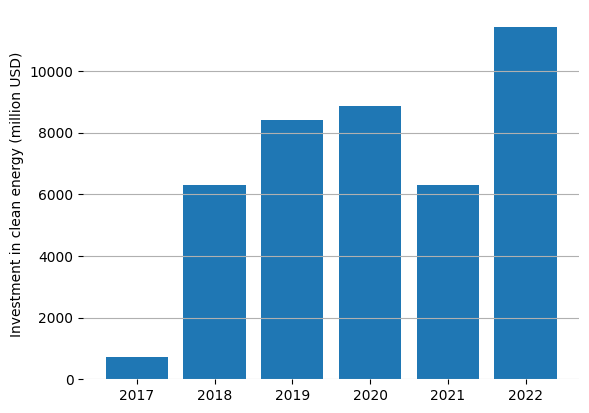
\includegraphics[width=0.7\linewidth]{assets/investment-clean.png}
    \caption{Investment in the Spanish clean energy sector, in million USD. \cite{renewable_energy_investments_2022}}
    \label{fig:investment-clean}
\end{figure}

This showcases the obvious interest there is in renewable energy in general in Spain. However, when talking about renewable energy it is very important to outline the different renewable energy resources and their corresponding technolgies \cite{ellabban_haitham_blaabjerg_2014}:
\begin{itemize}
    \item \textbf{Biomass}: Biomass energy is derived from organic materials, mainly plant and animal matter such as wood, agricultural crops, waste, and algae. It can be burned directly to produce heat and power a thermal power plant or it can be converted into biofuels like bioethanol or biodiesel. These fuels are then used in thermal power plants or for other uses like vehicle powering. It is very versatile with many of the main benefits of fossil fuels and can be used to reduce waste. However, sustainable sourcing of the biomass is critial, as otherwise it can lead to deforestation or other environmental issues.
    \item \textbf{Geothermal}: Geothermal energy harnesses the higher and more constant temperatures found deep below the Earth's surface, which originates from the planet's hot core due to the high pressure and the radioactive decay of different materials. Geothermal plants directly source hot water from underwater sources or pump fluids deep into the surface, heating it and retrieving it afterwards. This hot fluids can be used in a thermal power plant, as part of the cycle to preheat the working fluid or directly to heat up some buildings. It provides a constant and reliable energy supply not dependent on weather conditions and it has a samll land footprint. However, it is very location-specific, working best in regions with significant tectonic activity and with easily drillable materials in the ground. 
    \item \textbf{Hydropower}: Hydroelectric power is the power of flowing water. This water is generally stored in a dam and released to flow through turbines which generate electricity, although other systems which do not require dams and use water flowing in rivers are also possible. Worth mentioning are also pumped storage plants, which although are not strictly a renewable energy resource can be used as energy storage systems. Hydroelectric power has high efficiency and can provide electricty on demand with very short warm up periods, however the initial investment to build the dam is very costly, it cannot be placed anywhere and can disrupt the local ecosystems.
    \item \textbf{Marine}: Marine power leverages different sources of energy available in the seas and oceans. There are six main energy sources within this category:
    \begin{itemize}
        \item Wave: It transforms the kinetic energy of waves in their up and down movements into electrical energy.
        \item Tidal range: It leverages the difference in height between the high and low tide to generate electricity. 
        \item Tidal currents: It harnesses the horizontal currents caused by the rising and falling of the tide.
        \item Ocean currents: Similar to the previous source, however it leveraes currents not necessarily caused by tides, but caused by the dynamics of the ocean.
        \item OTEC: Ocean thermal energy conversion exploits the temperature difference between the warmer surface water and the colder deep water as the hot and cold sources of a thermal cycle to generate electrictiy.
        \item Salinity gradients: It leverages the difference in saline concentration between different areas of the ocean.
    \end{itemize}
    Many of these energy sources are still undergoing intensive research and developement and are still in the prototype and demonstration stage.
    \item \textbf{Solar}: Solar energy leverages the energy of solar radiation reaching us from the sun in several different ways:
    \begin{itemize}
        \item Photovoltaic: Solar PV systems directly convert the energy of the photons sent by the sun into direct current through the photoelectric effect \cite{einstein_1905}. The PV cells, generally made out of silicon, have an efficiency of around ~20\%. However they are very modular and can be produced at scale, helping achieve the tremendous drop in cost that has been seen during the last decade. 
        \item Thermal: Solar thermal power leverages the heating capacity of the solar radiation to harness its power. Although it is often used to directly heat up buildings, it can also be used to generate electricity. Concentrating solar power (CSP) produces electricity by concentrating the solar irradiance through mirrors and lenses to heat a liquid which is used in a thermal power cycle. 
    \end{itemize}
    \item \textbf{Wind}: Wind energy refers to the kinetic energy of wind currents. This energy can be transformed through wind turbines into electrical energy. Wind power is generally obtained through two different types of setups. There are on-shore and off-shore power plants, with the former being installed in land and the latter in seas or oceans near the coast. Off-shore installations have some advantages, like more powerful and constant wind, no land erosion and less landscape visual degradation, however its installation is more costly. 
\end{itemize}

As it can be seen, there are many different renewable energy resources and technologies that can be used to harness them and aid in the energy transition. However, not all of them are equivalent, with different technologies having different levels of maturity, profitability, capital requirements, etc. That is why generally the renewable energy mix is not very uniform. 

\begin{figure}[ht]
    \centering
    \captionsetup{justification=centering}
    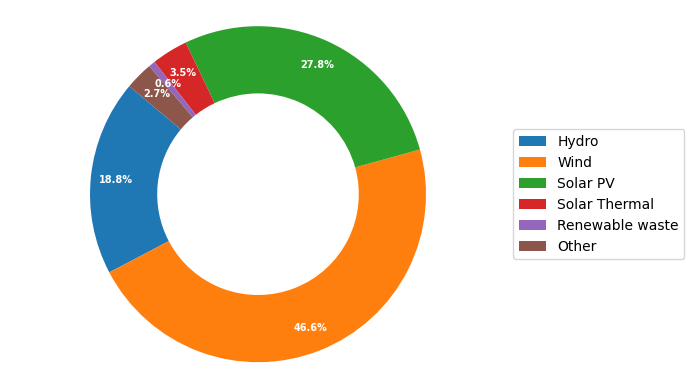
\includegraphics[width=0.7\linewidth]{assets/generation-mix.png}
    \caption{Generated renewable electricity mix in Spain in 2023. \cite{renewable_generation_reports_2023}}
    \label{fig:generation-mix}
\end{figure}

In \autoref{fig:generation-mix} it can be seen how solar, wind and hydro energy covers more than 95\% of the energy generation of 2023 -- as percentage of the total generation of 134.321 GWh of renewable energy -- while other sources like geothermal and biomass are almost negligible. 

\subsection{Motivation}
\label{sec:motivation}

In the previous section in \autoref{fig:generation-mix} a promising picture of the renewable energy generation in Spain could be seen, even more when the total generation is compared with the non-renewable generation of 132.486 GWh in Spain \cite{renewable_generation_reports_2023}, showing how renewable energy generation surpassed the 50\% mark.

However, the generation mix shown is also a source for concern. A 77.9\% of the total energy mix was produced through solar and wind energy. Solar and wind energy share some characteristics which lead to some grave challenges to the overall electrical system. Mainly, these characteristics and consequent challenges are:
\begin{itemize}
    \item \textbf{Variability}: These energy sources are intermittent. That is, one cannot choose to turn on a solar power plant at any moment, as its output depends on the solar input, which cannot be decided by the operator. This is translated into a very variable pattern of generation with high peaks and low troughs. 
    \\This variable pattern of production with rapid ramps leads to the need of having other power plants with also rapid ramp ups which can step up after a sudden fall of solar or wind production. These other plants also need to be very flexible to adapt to the wide changes in generation from these renewable resources.
    \item \textbf{Uncertainty}: Not only can these technologies not be discretionarily dispatched, but often it is difficult to know in advance what their behaviour will be at some point in the future. The further out into the future one looks, the less certain the sun and wind forecasts become, and thus the less certain the production output forecasts become.
    \\Many of the problems of variability are accentuated by the fact that this variability is uncertain. Given the grid players are uncertain about the renewable generation, large reserves need to be allocated in case the prediction fails. This in turn leads to more expensive electricity for the end consumer if the same level of reliability is required. 
    \item \textbf{Location specific}: The renewable resources are often geographically concentrated. For example, sun is more prominient in the south of Spain and wind around the coast. 
    \\Having many of these power plants geographically concentrated leads to several problems when all of them are producing at high outputs at the same time. Power lines connecting the renewable rich area with the rest can become overloaded forcing shutdowns and cutoffs. Furthermore, great voltage differences between areas in the grid can appear.
    \item \textbf{Generator technology}: The induction generators generally used in wind turbines or the inverters in solar power plants behave differently to the synchronous generators used in thermal power plants, which leads to problems in frequency control as will be outlined below. 
    \\This difference in generator technology leads to several problem. The first one being that these power plants are unable of providing the primary reserve matching supply and demand at the expense of frequency changes that synchronous generators supply automatically. Furthermore, these generators do not provide the same reactive power supply as the synchronous generators, and in the case of induction generators in wind turbines they in fact consume reactive power in order to function. It has also been hypothesized how these generators can lead to angular instability \cite{vittal_raja_ayyanar_2023}. The generators of wind turbines have also been shown to lead to problems of power quality due to the injection of different harmonics \cite{muljadi_butterfield_chacon_romanowitz_2006}. 
    \item \textbf{Low capacity factor}: Due to the variability in the resources, the capacity factor of installations leveraging sun and wind is generally lower to that of other non renewable technologies. 
\end{itemize}

Even more importantly, the greater the share of overall energy that comes from solar and wind sources the more pronounced these challenges will become. For more details regarding these characteristics and their consequences, refer to \cite{ahmed_fahad_2020}, \cite{kumar_pandey_sinha_2016} and \cite{steen_goop_2014}.

Grid operators need to consider these challenges at a short and medium term when opperating the grid, and plannificators should also consider it when planning the long term of the grid. 

The first two characteristics, the variability and uncertainty of these resources, leads in fact to a great problem in long term planning. When deciding where to locate which power plants and of what capacity, it is important to have accurate models of all resources. In fact, many of the optimization models used in long term planning require forecast models of these resources, which is very challenging due to the aforementioned characteristics. The lack of realistic and accurate models of solar and wind energy generation is precisely what this work aims to solve.

\subsection{Objective and scope}
\label{sec:objective-and-scope}
By looking at the overview of the wind and solar energy presented in \autoref{sec:motivation} \nameref{sec:motivation} and understanding the objectives and challenges of grid planners -- long term distribution of resources to ensure the grid's effectiveness and reliability -- the need for a model that can be used by these planners has become apparent. 

To be more precise, for such a model to be useful it must accurately represent the wind and solar energy generation marginal and joint distributions. The characteristics the model must fulfill are the following:
\begin{itemize}
    \item \textbf{Modeled variable}: The variable to be modeled is the hourly capacity factor of wind, solar PV and solar thermal energy generation. The capacity factor $f_t$ can be calcualted as 
    \begin{equation}
        \label{eq:capacity-factor}
        f_t=\frac{E_t}{P_t t}
    \end{equation}
    Where $E_t$ is the energy generated in a given timeframe, $P_t$ is the power output rating -- that is the rated installed capacity -- and $t$ is the length of the timeframe. As it can be seen, the capacity factor is a unitless ratio. 
    
    It has been chosen as the modeled variable due to having several beneficial characteristics. Numerically, $f_t \in \left[0,1\right]$ which makes it easier to model. It also is able to show the power generation without regarding the installed capacity. The installed capacity is often determined by policy decisions, awarded licenses or discretionary investment decisions by electricity companies and is thus harder to accurately model. The capacity factor however allows for an accurate representation of the generated power. 

    The hourly frequency has been chosen as it is short enough to allow for significant changes throughout the day, but is not short enough for noise to become a significant part of the variable. Furthermore, this is the frequency used by most market players, with the electrical market quoting hourly values for example. 

    The wind, solar PV and solar thermal capacity factors have been chosen as independent variables because the three of them have significantly different driving factors, making them have different dynamics that can be captured by individual models. Even the solar PV and solar thermal have different dynamics, thanks to the inertia provided by the storage of heat in solar thermal power. 
    \item \textbf{Input variables}: The only exogenous variable that will be used in all models are the historical values of these capacity factors and temporal variables such as the month or hour. A purely time series approach has been taken, as opposed to other physical approaches that leverage weather forecasts. The intuition for this decision is that the information provided by the weather or any other significant variable should be integrated in the capacity factor, and relying on other external variables forces a two step approach where a model for those variables needs to be created and then a model for the capacity factor needs to be created, as there are no accurate forecasts for any of the other possible exogenous variables with a long enough timeframe. 
    \item \textbf{Geographical scope}: The capacity factor will be that of the national Spanish power system. 
    \item \textbf{Temporal scope}: The model should be able to forecast the capacity factor for a period of 1 to 10 years into the future, with hourly values. 
    \item \textbf{Methodological scope}: Statistical, machine learning and deep learning models will be studied as candidates to modeling this variable. 
\end{itemize}

% \subsection{Study structure}

\newpage
\section{Literature Review}
Given the great and increasing importance of renewable energy, it is of no surprise that many scholars have already shown great interest in all aspects surrounding it. From the development of the technology, to the analysis of its use, there is an incredible amount of papers regarding the topic. 
% \subsection{Overview of renewable energy in Spain}
% \subsection{Solar power generation}
% \subsection{Wind power generation}
% \subsection{Modeling techniques}
% \subsection{Performance metrics for model evaluation}
\newpage
\section{Data Description}
\label{sec:data-description}
\subsection{Data Sources}
The datasets needed for the exploration of the time series and the fitting of the models have been obtained from the ESIOS -- System Operator's Electronic Information System. This is an online portal where the System Operator, the REE -- Spanish Electrical Grid -- uploads all relevant information for the operation of the grid. 

In order to accomplish everything outlined in \autoref{sec:objective-and-scope} six different datasets are needed. These datasets are:
\begin{itemize}
    \item Real time wind energy hourly generation
    \item Real time solar PV energy hourly generation
    \item Real time solar thermal energy hourly generation
    \item Wind energy monthly installed capacity
    \item Solar PV energy monthly installed capacity
    \item Solar thermal energy monthly installed capacity
\end{itemize}

%\href{https://www.esios.ree.es/es/analisis/551?vis=1&start_date=26-08-2024T00%3A00&end_date=26-08-2024T23%3A55&compare_start_date=25-08-2024T00%3A00&groupby=minutes5}{https://www.esios.ree.es/es/analisis/551}
%\href{https://www.esios.ree.es/es/analisis/1295?vis=1&start_date=26-08-2024T00%3A00&end_date=26-08-2024T23%3A55&compare_start_date=25-08-2024T00%3A00&groupby=minutes5}{https://www.esios.ree.es/es/analisis/1295}
%\href{https://www.esios.ree.es/es/analisis/1294?vis=1&start_date=26-08-2024T00%3A00&end_date=26-08-2024T23%3A55&compare_start_date=25-08-2024T00%3A00&groupby=minutes5}{https://www.esios.ree.es/es/analisis/1294}

\subsection{Data Preprocessing}
The obtained datasets are already very clean, so no missing or obviously wrong values were found on any of them. The installed capacity is obtained on a monthly basis as there is not any lower granularity in the ESIOS portal. With this datasets, the capacity factor is obtained as explained in equation \eqref{eq:capacity-factor} by dividing the generated electricity by the installed capacity times the period time frame. The time frame in this case is always one hour. Like this the hourly capacity factor for the Spanish electrical system for the three different technologies is obtained. Note that the data obtained spans from mid 2015 until end of 2023, since no previous data is available. 

\subsection{Exploratory data analysis}

Now that it is well understood where the data comes from, an initial analysis of the data to understand what the capacity factor of each looks like will be performed. 

\subsubsection{Initial visualization}
The first variable to be visualized will be that of the solar PV capacity factor, which can be seen in 
\begin{figure}[ht]
    \centering
    \captionsetup{justification=centering}
    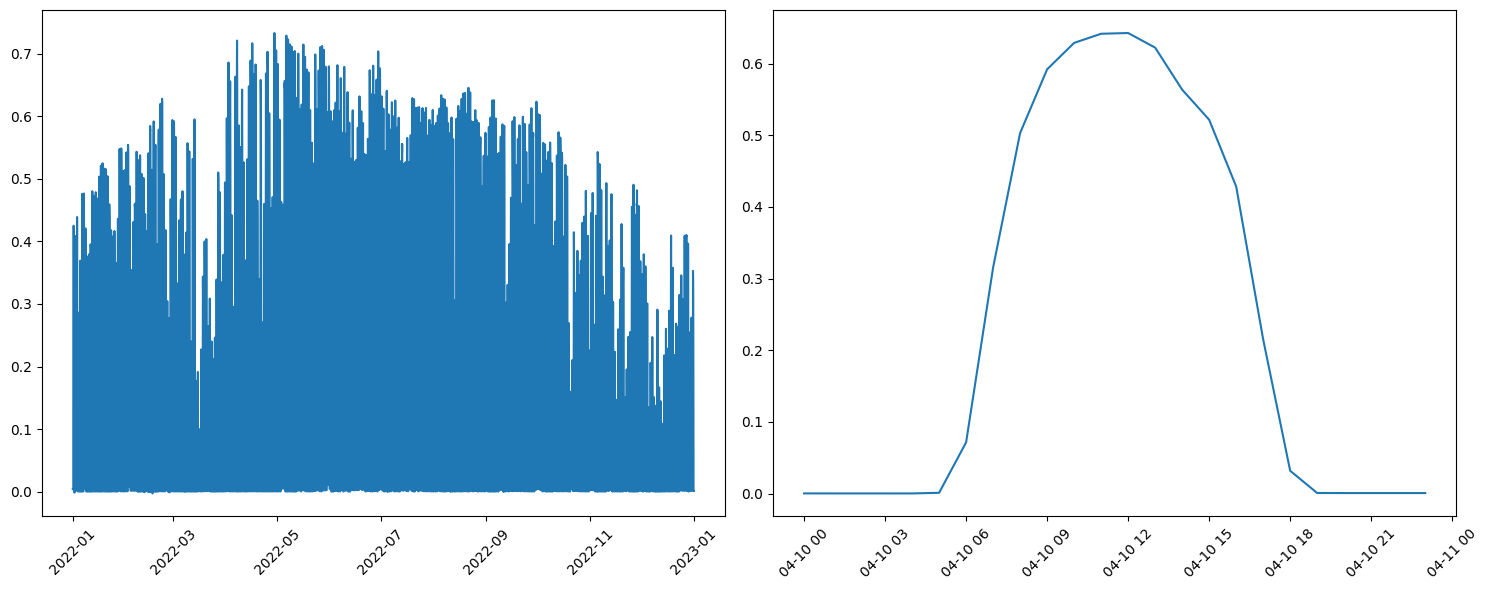
\includegraphics[width=\linewidth]{assets/spv-year-day.png}
    \caption{Yearly and daily profiles of the solar PV capacity factor, taken for 2022 and the 10\textsuperscript{th} April 2022 respectively.}
    \label{fig:spv-year-day}
\end{figure}

The main features of the series can be well visualized here. The yearly seasonality is very clear, with higher peak values in summer and lower peak values in winter, although this is altered by periods of lower sunlight where peaks are reduced below the typical seasonal peak, like at the beginning of March. The daily pattern is also very clear, with values of practically zero -- it is not exactly zero due to some background light and noise in the measurement -- at night and a generation in accordance with the position of the sun in its ecliptic. 

The solar thermal profile, although belonging to the same renewable resource as the solar PV, is slightly different. 
\begin{figure}[ht]
    \centering
    \captionsetup{justification=centering}
    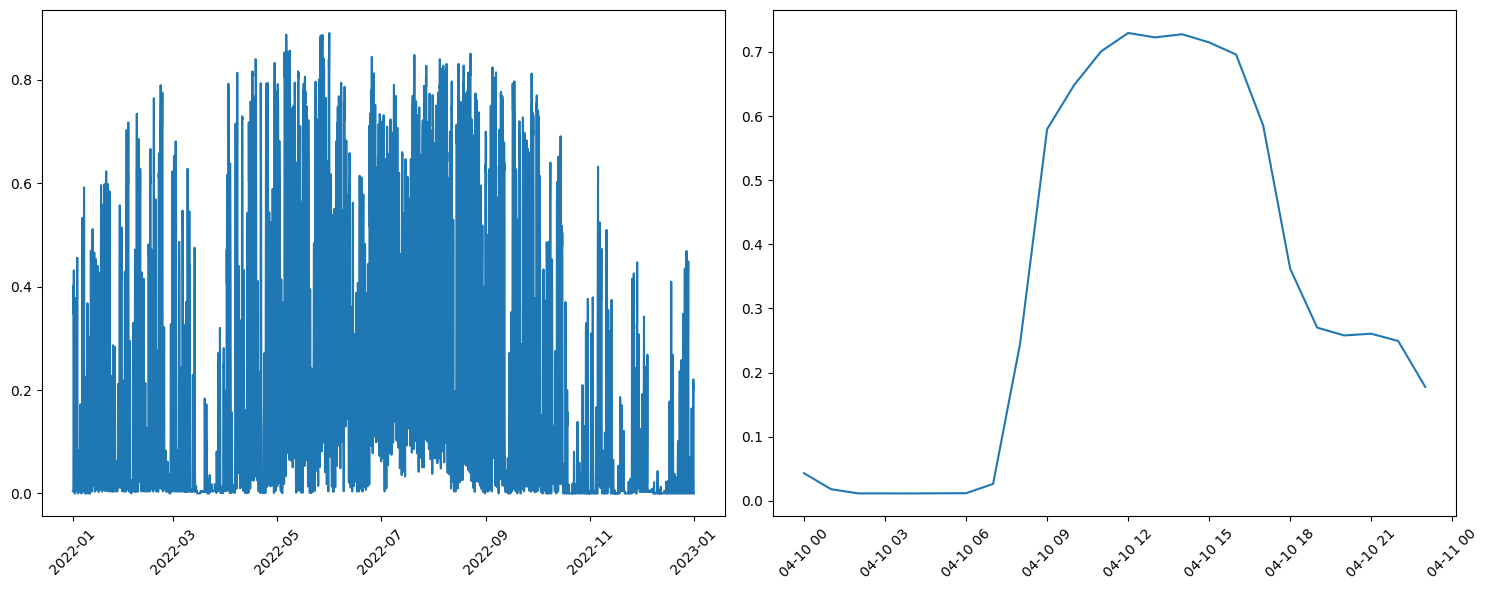
\includegraphics[width=\linewidth]{assets/st-year-day.png}
    \caption{Yearly and daily profiles of the solar thermal capacity factor, taken for 2022 and the 10\textsuperscript{th} April 2022 respectively.}
    \label{fig:st-year-day}
\end{figure}

Several differences between these profiles shown in \autoref{fig:st-year-day} and the previous ones are apparent. The yearly pattern, even though it follows roughly the same seasonality with higher peaks in summer is much more volatile than that of the solar PV. Furthermore, there are whole periods of several days where generation does not go to zero, due to the inertia of the thermal system. The highest peaks are also whigher for the solar thermal, reaching generation values much closer to its rated capacity in the summer than the solar PV. In the daily pattern the mentioned inertia can be clearly seen, where appart from the general sinusoidal throughout the day it can be seen how generation remains above zero at night.

\begin{figure}[ht]
    \centering
    \captionsetup{justification=centering}
    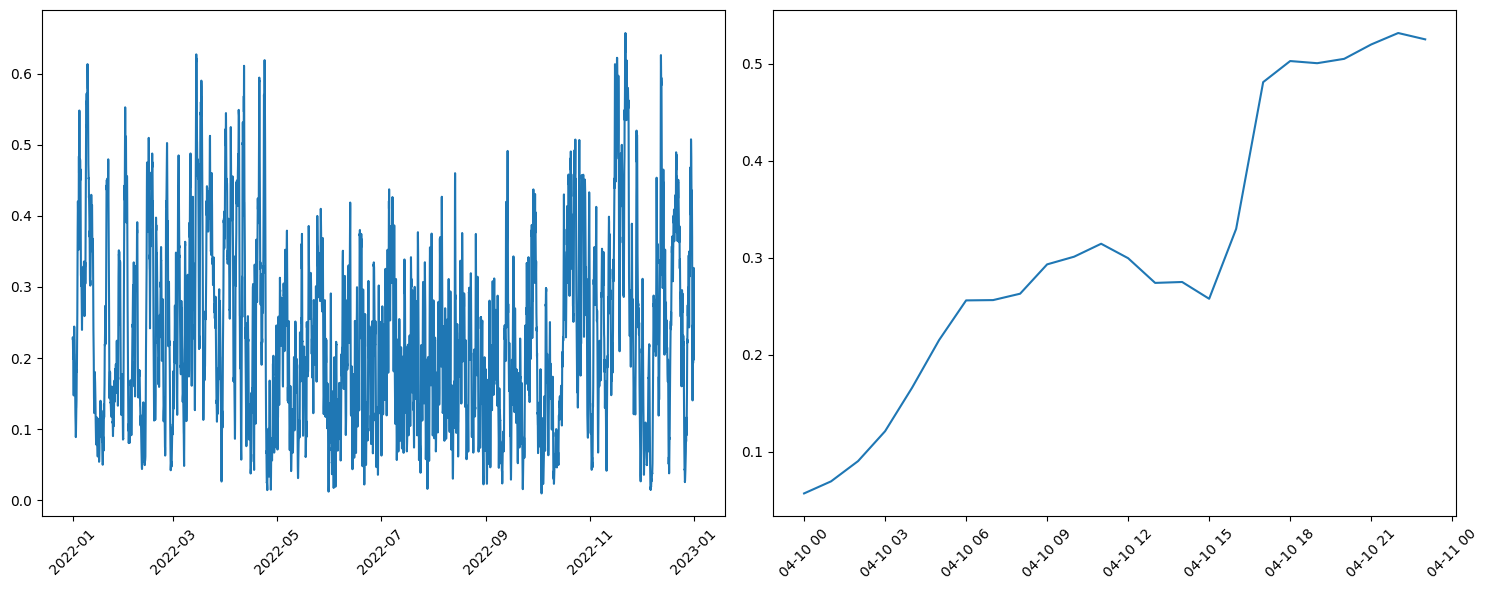
\includegraphics[width=\linewidth]{assets/w-year-day.png}
    \caption{Yearly and daily profiles of the wind capacity factor, taken for 2022 and the 10\textsuperscript{th} April 2022 respectively.}
    \label{fig:w-year-day}
\end{figure}

The wind profile shown in \autoref{fig:w-year-day} is the most different of the three. The yearly profile is the most volatile of the three, with less of a clear seasonal pattern although it can be seen how the mean values in summer seem to be lower than those in the winter. In the daily profile there are not any obvious patterns which can be seen at first view. 

\subsubsection{Individual statistical characteristics}
After an initial view of the general time series for the three variables, a deeper look at the main statistical properties of these individual series is pertinent. For this deeper look a KDE and cumulative KDE will be shown and the main moments will be calculated. 

The Kernel Density Estimate (KDE) is a non-parametric way of estimating the probability density function (PDF) of a random variable. It works by placing a kernel -- that is a smooth, symmetric function -- at each data point and then summing these kernels to produce a smooth estimate of the PDF. In more precise terms, the estimation of the PDF at $x$ denoted by $\hat{f}\left(x\right)$ is calculated as
\begin{equation}
    \hat{f}\left(x\right)=\frac{1}{nh}\sum^n_{i=1}K\left(\frac{x-x_i}{h}\right)
\end{equation}

where $n$ is the number of datapoints, $K\left(\cdot\right)$ is the kernel function, $h$ is the bandwidth -- a parameter used to approximate the width of the kernel and thus how smooth or sensitive to individual points the estimation is -- and $x_i$ are the individual datapoints.

The chosen kernel function has been the Gaussian kernel, which is calculated as 
\begin{equation}
    K\left(x\right)=\frac{1}{\sqrt{2\pi}}\exp{-\frac{1}{2}x^2}
\end{equation}

The method selected for estimating the optimal bandwidth has been the method outlined in \cite{scott_1979}. 

The cumulative KDE is an analogous method used for calculating the cumulative density function (CDF) instead of the PDF. It is calculated as
\begin{equation}
    \label{eq:cumulative-kde}
    \hat{F}\left(x\right)=\frac{1}{n}\sum^n_{i=1}\int_{-\infty}^{x}\frac{1}{h}K\left(\frac{t-x_i}{h}\right)dt
\end{equation}

The KDE and cumulative KDE of all three variables can be seen in \autoref{fig:kde-triple}

\begin{figure}[ht]
    \centering
    \captionsetup{justification=centering}
    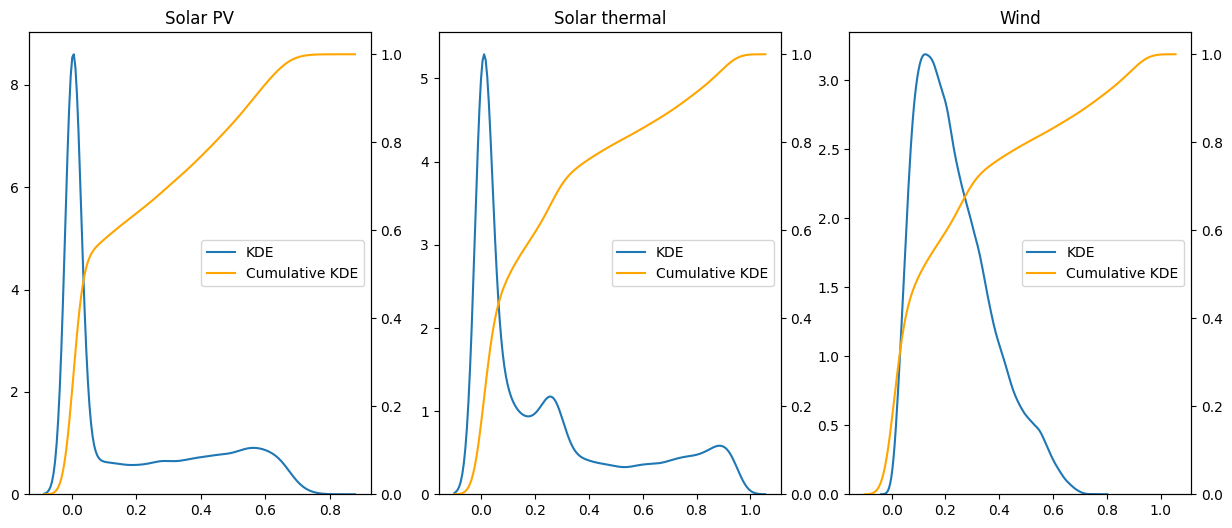
\includegraphics[width=\linewidth]{assets/kde-triple.png}
    \caption{KDE and cumulative KDE of the three capacity factors}
    \label{fig:kde-triple}
\end{figure}

Several observations can be made regarding these plots. First of all, the high density of zero like values in both solar plots is clear, with an even higher denisty in the solar PV. In fact it can be seen how both KDE have non zero values for x values below zero, however this only happens due to the symmetry and width of the gaussian kernel, which for the points at zero sums some value for points below zero. Appart from the mode at zero, both plots have another peak near their maximum value, at around 0.6 and 0.9 for the solar PV and solar thermal respectively. This is due to the shape of the solar ecliptic, where the sun remains at its highest point for longer than it is at any given point during ascent or descent. The solar thermal PDF also has a significant peak at around 0.3, probably due to this being the power at which the power plants runs with the stored heat at night. This is in fact the point where the daily curve in \autoref{fig:st-year-day} can be seen operating at night. As for the wind PDF and CDF, it is a much smoother plot, with the mode around 0.1 and then slowly and gradually tapers of. 

In order to have a more quantitative view of these distributions, metrics relating to the first four moments are shown in \autoref{table:main-moments}

\begin{table}[ht]
    \centering
    \begin{tabular}{rccc}
        \toprule
        Metric & \multicolumn{3}{c}{Value} \\ 
        \cmidrule(lr){2-4}
            & Solar PV & Solar Thermal & Wind \\
        \midrule
        Mean & 0.18 & 0.24 & 0.23 \\
        Standard Deviation & 0.23 & 0.29 & 0.14 \\
        Skew & 0.88 & 1.12 & 0.78 \\
        Kurtosis & -0.79 & -0.08 & 0.01 \\
        \bottomrule
    \end{tabular}
    \caption{Main moments of the three capacity factors}
    \label{table:main-moments}
\end{table}

Through these measures it can be seen how some of the intuitions obtained when looking at the time series plot of the different capacity factors were wrong. For example, the wind capacity factor is not the most volatile as it seemed, but in fact has the lowest standard deviation. This could be however due to the high variability of the solar profile, and taking away the seasonality of the three variables these metrics could be different.

\subsubsection{Lagged relationships}
\label{sec:lagged-relationships}
Another key factor about the three series is their seasonality and how a given value at $t$ is influenced by past values at $t-1, t-2...$. In order to explore these relationships, two different metrics will be used. 

The first one is the the autocorrelation. While correlation as expressed by the Pearson correlation coefficient is generally calculated like
\begin{equation}
    \rho{\left(X,Y\right)}=\frac{\text{cov}\left(X,Y\right)}{\sigma_X\sigma_Y}=\frac{\sum^n_{i=1}\left(x_i-\bar{x}\right)\left(y_i-\bar{y}\right)}{\sqrt{\sum^n_{i=1}\left(x_i-\bar{x}\right)^2}\sqrt{\sum^n_{i=1}\left(y_i-\bar{y}\right)^2}}
\end{equation} 

The autocorrelation function of a series quantifies the correlation of a series with lagged values of itself at different lags. For a given lag $k$ it is thus calculated like
\begin{equation}
    \label{eq:acf}
    ACF\left(k\right)=\frac{\sum^{N-k}_{t=1}\left(x_t-\bar{x}\right)\left(x_{t+k}-\bar{x}\right)}{\sum^{N}_{t=1}\left(x_t-\bar{x}\right)^2}
\end{equation} 

The correlation coefficient has some known drawbacks however. It only measures linear relationships, so any dependence appart from this very simple relationship cannot be captured through a high correlation coefficient. That is what the new correlation coefficient proposed by \cite{correlation_2021} aims to solve, and why it has been included here. This new correlation coefficient, capable of capturing non linear relationships and with some very interesting statistical properties is calculated as 
\begin{equation}
    \xi{\left(X,Y\right)}=1-\frac{3\sum_{i=1}^{n-1}\left|r_{i+1}-r_i\right|}{n^2-1}
\end{equation}

Where the given pairs $\left(x_1,y_1\right), \left(x_2,y_2\right)...\left(x_n,y_n\right)$ have been aranged so that $x_1 \leq...\leq x_n$. Here $r_i$ denotes the rank of $y_i$. That is, the number of $j$ such that $y_j\leq y_i$. If there are ties among the $x$ values, the formula is slightly different, however with the capacity factor being a continuous variable it can be assumed that no ties will be present. Finally, note how even though $\rho \in \left[-1,1\right]$ the new correlation coefficient makes no distinction between positive and negative relationships and $\xi \in \left[0,1\right]$.

With this new correlation coefficient, a new autocorrelation function is constructed in the same way as in \eqref{eq:acf}, calculating the correlation of the series with its lagged values for each lag. The following figure shows both autocorrelation functions for the three series. 

\begin{figure}[ht]
    \centering
    \captionsetup{justification=centering}
    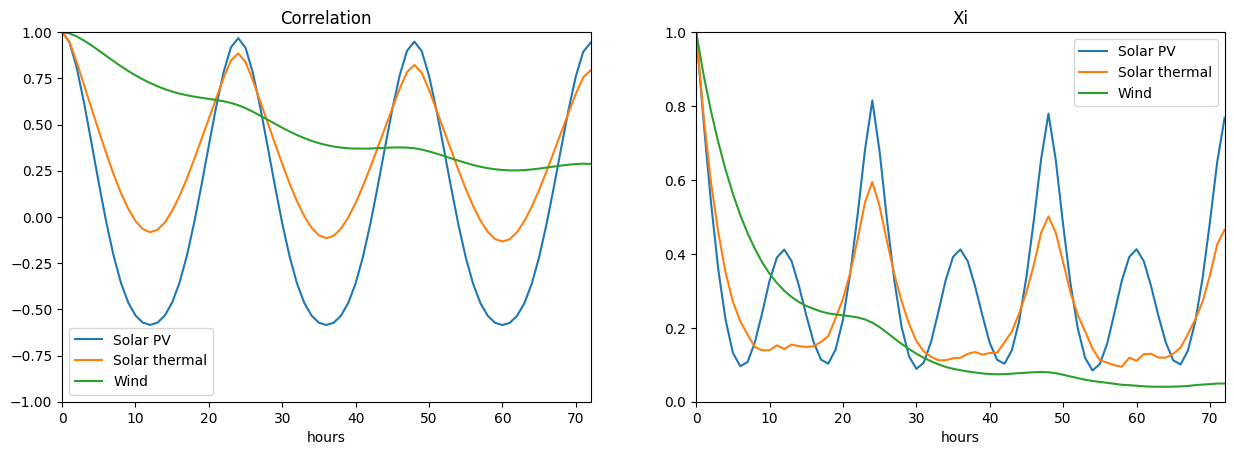
\includegraphics[width=\linewidth]{assets/autocorrelation.png}
    \caption{Autocorrelation functions with the two correlation coefficients for the three capacity factors at different hourly lags}
    \label{fig:autocorrelation}
\end{figure}

Several observations can be made from the two autocorrelation functions in \autoref{fig:autocorrelation}. The seasonality in both solar series is again made apparent, with high autocorrelations at the 24, 48 and 72 hour mark showcasing the importance of the previous days' values at the same hour for a given day, but also at the 12, 36 and 60 hour mark. This second autocorrelation, negative in the case of pearson correlation, denotes the relationship between opposite moments of the day between different days. It is also noted how the correlation in the case of the solar PV is much more persistent, with the correlation peaks remaining more or less constant for the three days, while for the solar thermal this correlation tapers off a little bit faster. It is also interesting to see how the correlation at the 12, 36 and 60 hour mark is a lot lower for the solar thermal, showcasing how this relatinoship between values at a lag of 12 hours practically -- although not completely -- disappears, again due to the inertia of the thermal system which makes the solar thermal cycle less related to the sun's trayectory. As for the wind autocorrelation functions, it is much more linear and smooth, with the relevance of past values reducing gradually as the hours go by. There is a slight daily seasonality as well with the autocorrealtion at daily lags being slightly above what could be expected from the linear trend. However, this has a practically negligible relevance compared with the solar series. In fact, for the wind capacity factor it can be seen how the immediately previous values have much higher significance, while previous lags at the daily or semidaily periods hold much less significance. 

\textcolor{red}{INCLUDE SEASONAL LAGS?}
\subsubsection{Seasonal statistical characteristics}
Even though the characteristics shown in previous sections already provides very significant information, it seems like many of these characteristics may be seasonally dependent. That is, they may not be the same in summer and in winter, or at night and during the day. That is why the previous analyses will be performed again but seasonally separating the datasets. Both daily and yearly splits will be done, where "day" is the period from 06:00 to 18:00 UTC and "night" is the period from 18:00 to 06:00 UTC. On the yearly split and taking into account the day's number within a year, spring goes from the 3\textsuperscript{rd} to the 5\textsuperscript{th} month, summer from the 6\textsuperscript{th} to the 8\textsuperscript{th}, autoumn from the 9\textsuperscript{th} to the 11\textsuperscript{th} and winter from the 12\textsuperscript{th} to the 2\textsuperscript{nd}, both inclusive in all cases. Note how these are metereological seasons, and not astronomical seasons based on the solstices and equinoxes. 

The yearly seasonal breakdown can be seen in \autoref{fig:kde-triple-seasonal}. 

\begin{figure}[ht]
    \centering
    \captionsetup{justification=centering}
    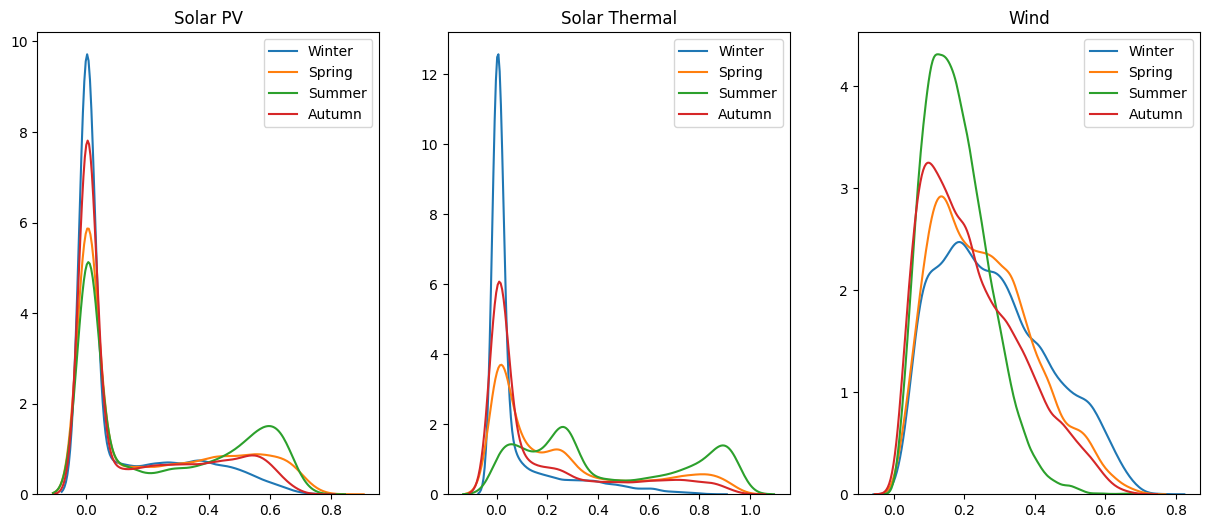
\includegraphics[width=\linewidth]{assets/kde-triple-seasonal.png}
    \caption{KDE plot for the three capacity factors for the different yearly seasons}
    \label{fig:kde-triple-seasonal}
\end{figure}

For the solar PV it can be seen how on one extreme in winter the concentration of zeroes is highest, with very low density in the previously seen peak at 0.6, while in the summer the concentration of zeroes is still high -- due to the night hours -- but much less, and the peak at 0.6 can be clearly seen. Spring and autumn are found in between these values, with spring having a density of zeroes slightly above summer but a much lower peak at 0.6. For solar thermal the difference in density at zero is much higher, with winter having higher density and the rest of the seasons having a much lower one. In fact, for summer density at zero es very low, much more than other peaks. The peak at 0.9 can again only be seen in the summer, and the peak at 0.3 can be seen mainly for summer but also slightly for spring. As for the wind distribution, the summer season seems to be the one with the lowest volatility and lowest mean, while winter has the widest PDF and apparently mean.  

\begin{figure}[ht]
    \centering
    \captionsetup{justification=centering}
    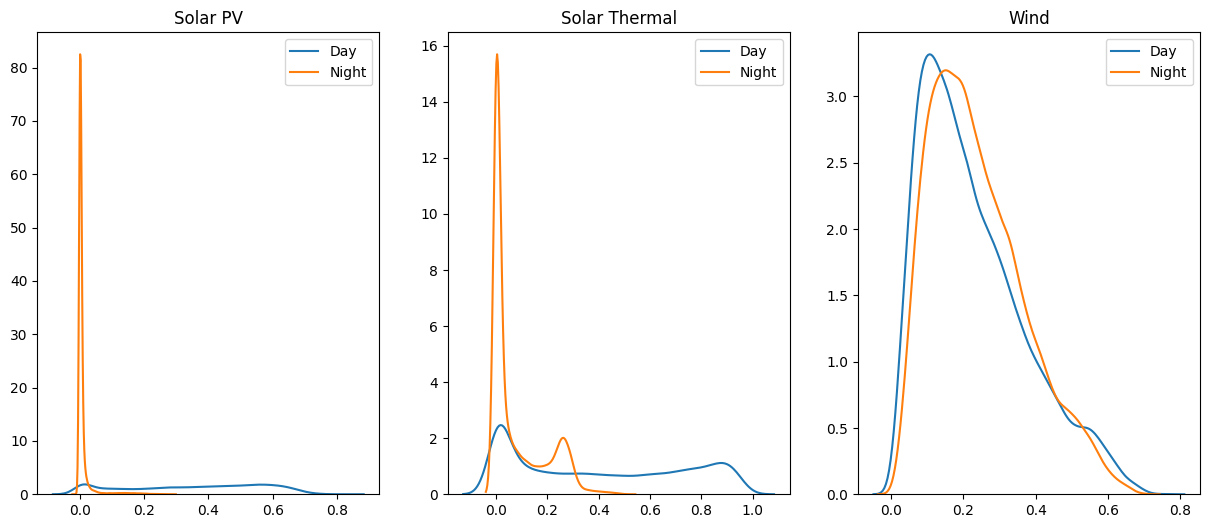
\includegraphics[width=\linewidth]{assets/kde-triple-daily.png}
    \caption{KDE plot for the three capacity factors for the different daily periods}
    \label{fig:kde-triple-daily}
\end{figure}

In \autoref{fig:kde-triple-daily} a similar representation for the KDE can be seen but for the split between night and day. For solar PV the plot is not very interesting, with the night having all its density at the zero point, with the day density having a slight peak at zero -- as the exact times for sunset and sunrise vary during the year and the period defined here as "day" can in fact have some night time -- and the already known one at 0.6. For solar thermal it can be seen how the peak at 0.9 is exclusively a day time fenomenon while the peak at 0.3 is a night time fenomenon, confirming the hypothesis that this was the power generated at night with the stored heat from the day. For the wind, it can be seen how the difference between day and night is practically negligible, with day exhibiting a slightly more "summer" like behaviour -- that is, slightly less volatile and lower mean. 

\subsubsection{Multivariate analysis}
\label{sec:multivariate-analysis}
Up until this point every analysis has been performed on a per variable basis, examining their individual properties. However, when thinking about the true implications for the power grid it becomes clear that the joint characteristics are also fundamental. For a given wind and solar distributions, the consequences of the grid are not the same if peaks in both happen at the same time or if they complement each other. That is why the joint characteristics will be studied, and they will mainly be studied through cross correlation and through copula analysis. Some other analysis, like through Granger causality as outlined in \cite{granger_1969} were attempted, but no new relevant information that wasn't uncovered through cross correlation was found. 

Cross correlation follows a principle very similar to the autocorrelation, but instead of measuring the correlation of a series with lagged versions of itself, the correlation of a variable with lagged versions of a different variable are measured. That way, something similar to the predictive value of the second variable on the first can be understood. Again, the two different correlation coefficients already explained were used. Note how for Person's correlation the relationship for $\left(X,Y\right)$ is the same as for $\left(Y,X\right)$. However, when using lagged values the correlation does depend on which variable is lagged. for the new correlation coefficient the directionality matters, as the effect of one variable on a second is not the same as that of the second on the first one. 

In \autoref{fig:cross-correlation} the lagged cross correlation between each pair of variables can be seen. For each of the three variables, it is shown how the lagged versions of the other two are correlated to the given variable, for each of the two correlation coefficients. 

\begin{figure}[ht]
    \centering
    \captionsetup{justification=centering}
    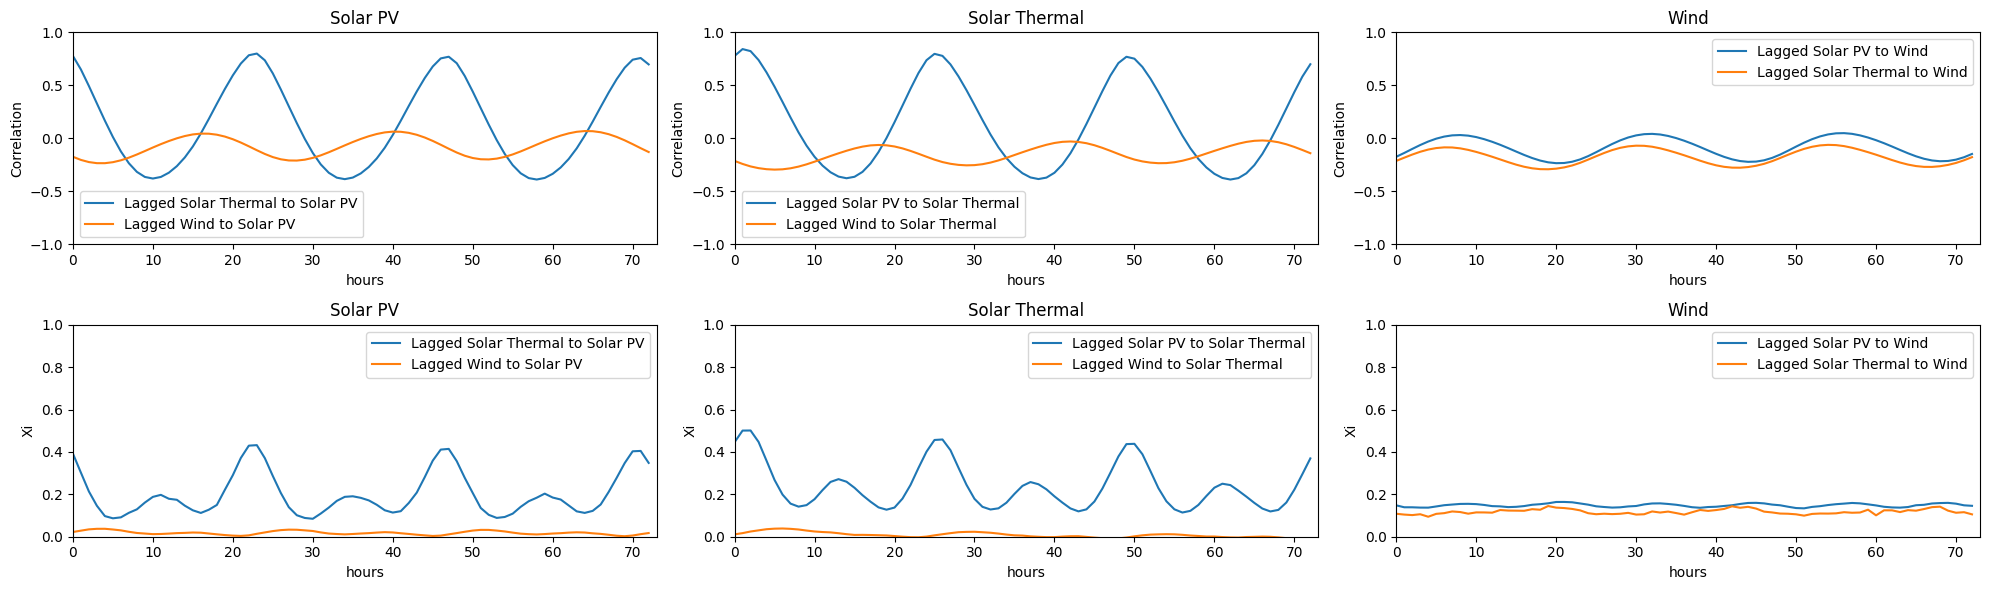
\includegraphics[width=\linewidth]{assets/cross-correlation.png}
    \caption{Lagged cross correlation between each pair of capacity factors}
    \label{fig:cross-correlation}
\end{figure}

The similarity between the solar PV and solar thermal is clearly shown, with high correlations in both directions. Interestingly, the solar thermal capacity factor is more highly correlated with the 1-lag solar PV than with the simultaneous solar PV, probably due to the time it takes for the working fluid to be heated up, while the PV cells are able to convert that sunlight into power instantaneously. The second notable observation is that the predictive power of solar on wind seems to be higher than that of wind on any solar when looking at the Xi. Also, that correlation of the two lagged solar variables does not seem to decay for the examined 3 day period, and a very slight lag effect is seen where the daily seasonality of the sunlight is seen in the correlation, with wind being negatively correlated to simultaneous solar power but positively correlated to solar power at a lag of around 8 hours. 

\textcolor{red}{INCLUDE SEASONAL CROSS LAGS?}

The second method used to see how the three variables compare to each other will be using copulas. Copulas are multivariate functions used to model the dependence between several random variables. Consider the random vector $(X_1,X_2,X_3)$ representing the observations of capacity factor for solar PV, solar thermal and wind energy for a given point in time. The marginal CDF of each of the variables is represented as $F_i\left(x\right)=P\left(X_i\leq x\right)$, which when applied to the random vector yields the marginals $\left(U_1,U_2,U_3\right)=\left(F_1\left(X_1\right),F_2\left(X_2\right),F_3\left(X_3\right)\right)\in \left[0,1\right]^3$. The copula $C(\cdot)$ is the joint cumulative distribution function such that 
\begin{equation}
    C\left(u_1,u_2,u_3\right)=P\left(U_1\leq u_1,U_2\leq u_2,U_3\leq u_3\right)
\end{equation}

The copula contains all information on the dependence structure between the three series, while the marginal cumulative distribution functions contain all inforamtion on the marginal distribution of the variables. 

In this analysis, the marginal CDF used has been the gaussian cumulative KDE outlined in \eqref{eq:cumulative-kde}. The copula used has been a gaussian copula, which relies on the multivariate normal distribution.

For the fitting process, a cumulative gaussian KDE is fitted for each of the variables and then the univariate values are transformed according to that CDF. Then, the normal percent point function (PPF) -- the inverse of the CDF -- is applied to transformed variable to normalize it. Then, a multivariate gaussian is fitted on the normalized data. 

The correlation matrix of the gaussian copula can be seen in \autoref{table:copula-correlation-matrix}.

\begin{table}[ht]
    \centering
    \begin{tabular}{r|ccc}
        & Solar PV & Solar thermal & Wind \\
        \midrule
        Solar PV & 1.00 & 0.72 & -0.19 \\
        Solar thermal & 0.72 & 1.00 & -0.23 \\
        Wind & -0.19 & -0.23 & 1.00 \\
    \end{tabular}
    \caption{Correlation matrix of the gaussian copula with gaussian KDE marginals}
    \label{table:copula-correlation-matrix}
\end{table}

It can be seen how in the copula representation the strong positive correlation between both solar series and the negative correlation between wind and both solar series still stands. 

% \subsubsection{Extreme value analysis}
% \textcolor{red}{NECESSARY HERE(?)}
\newpage
\section{Methodology}
In this section several points regarding the methodology used in the work will be presented. The general approach taken to modeling, as well as the models themselves will be explained. The metrics used to evaluate the goodness of fit of the different models will also be presented. 

\subsection{Overview of modeling approach}
In order to understand why the models that will be presented below have been chosen and why the evaluation metrics have been chosen, it is worth first taking a look at the requirements of the modeling task and the general criteria that determine what a good result is.

\subsubsection{Modeling task characteristics}
\label{s:modeling-task-characteristics}
The general technical characteristics of the task, from the objectives and the time series characteristics already explored are the following:
\begin{itemize}
    \item \textbf{Modeling horizon}: The horizon to be modeled is of between 1 and 10 years, or between 8.760 and 87.600 hourly timesteps. 
    \item \textbf{Available data}: The data available for the training and testing tasks consists of slightly below 10 years of data, or slightly below 87.600 observations. This data has been consistently recorded at a 1 hour timestep interval.
    \item \textbf{Seasonality}: There has been found to be high seasonality, both at the daily and yearly frequencies. 
    \item \textbf{Exogenous variables}: A certain predictive power of some series with respect to the others has been found. Thus the capacity of incorporating the use of exogenous variables or multivariate modeling aproaches are specially interesting. 
    \item \textbf{Extreme values}: There is a special interest in having accurate modeling of the extreme values, specially in the wind capacity factor.
    \item \textbf{Pointwise forecast}: The forecasts produced by the model can be pointwise predictions, there is no need to produce probabilistic forecasts for each timestep.
\end{itemize}

\subsubsection{Modeling criteria}
Starting with the objectives already outlined in the section called \nameref{sec:objective-and-scope}, here these objectives will be broken down into more specific criteria that the best model must aim to meet in the best possible way. The specific characteristics the model must meet are the following:
\begin{itemize}
    \item \textbf{Seasonality}: The chosen models must be able of incorporating seasonality into its forecast. 
    \item \textbf{Multiple variables}: The chosen models should be able to incorporate multiple variables, be it through a multivariate modeling, through historical exogenous variables and/or through future exogenous variables. Through the modeling task it will be made apparent wether incorporating the information of the other series helps in modeling a given series.
    \item \textbf{Complex relationships}: The temporal relationships of a series with itself and the relationships of a series with the other variables are probably more complex than linear relationships. That is why a model capable of incorporating complex non linear temporal and intervariate relationships will probably have an advantage.
    \item \textbf{Multiperiod modeling}: As it has already been mentioned, the modeling period will encompass between 8.760 and 87.600 timesteps. The model must be able to create such forecasts. But going further, if the prediction is created by autoregressively estimating the next step, there is a compounding in errors over time \cite{educing_error_propagation_long}. By estimating multiple timesteps in one prediction pass, the number of autoregressive steps can be reduced and with it the compounding of errors can be reduced too. Therefore, models with bigger single-step prediction window should have an advantage.
    \item \textbf{Long and short term temporal relationships}: The model must be able to incorporate both long term and short term temporal relationships.
    \item \textbf{Robustness}: The model must be resistant to overfitting, given the parameter size of some of the models and the number of available training datapoints. 
    \item \textbf{Extreme value accuracy}: The model must be specially sensitive to extreme values, be it through the flexibility of incorporating a custom loss function or through its intrinsic characteristics.
    \item \textbf{Computational efficiency}: Given the long modeling horizon, the model must be efficient both in prediction time and in memory used when training and when incorporating historical data in prediction.
\end{itemize}
\subsection{Models}
\label{s:models}
Now that the criteria used to select potential models has been outlined, the different models that will be evaluated can be presented. These models have been divided by model family or type. Here below, the different model types and each of the models and their characteristics and main working principles are explained. 
\subsubsection{Statistical models}
These models are based on classical statistical methods to analyze and predict temporal series. They use techniques like regression analysis, autocorrelation and spectral analysis to model and forecast temporal variables. The ones that will be used here are:
\begin{itemize}
    \item \textbf{Linear Regression}: This is the most simple model and it will be used as a naive benchmark. It models a given capacity factor value for one of the series as a linear combination of several exogenous variables. In this case, those variables are the values of fourier sine and cosine terms, some lagged values of the given time series and some lagged values of other time series, which in this case will be the other capacity factors. The main parameters of the model are thus:
    \begin{itemize}
        \item Seasonal frequencies: That is the frequencies for which the fourier terms will be calculated. It can be daily, yearly, both, etc.
        \item Fourier harmonics: For each of the seasonalities, several harmonics of fourier terms can be calculated, creating more nuanced patterns the more harmonics are added.
        \item Autoregressive order: That is, what lags of the modeled series to incorporate.
        \item Exogenous lags: That is, what lags of the other two series to incorporate. 
    \end{itemize}
    The mathematical formulation for the model thus is:
    \begin{multline}
        Y_t=\beta_0 + \sum_{\tau}\sum_{k}\left[\gamma_{\tau,k}\sin\left(\frac{2\pi k t}{\tau}\right) + \delta_{\tau,k}\cos\left(\frac{2\pi k t}{\tau}\right)\right] +\\+ \sum_l \phi_l Y_{t-l} + \sum_v\sum_p\theta_{v,p}X_{v,t-p} + \epsilon_t
    \end{multline}
    where $\tau$ is each of the seasonality periods, $k$ is each of the fourier harmonics, $l$ is each of the self lags, $v$ is each of the other two capacity factors and $p$ is each of the lags used for the two other capacity factors.
    
    This model opperates on several assumptions which are worth mentioning. The first is that all relationships -- those with the seasonal terms, with lagged values, with the other capacity factors, etc. -- are assumed to be linear. The error term $\epsilon_t$ is assumed to be independent and identically distributed (i.i.d.) with constant variance (homocedastic) and gaussian, although there is no evidence that this is true. 
    \item \textbf{ARIMAX}: The AutoRegressive Integrated Moving Average with eXogenous variables model is an extension to the previous model. It incorporates both autoregressive and moving average components to the endogenous time series and allows for time  integration, which extends the purely autoregressive view in the previous model, as well as some exogneous variables. It provides a more complex representation of the relationship of the time series with its lagged values than the linear regression model presented above. To the previously presented parameter, these new ones are added:
    \begin{itemize}
        \item Integration order: This represents the number of times the endogenous time series is differentiated. 
        \item Moving average order: That is, what moving average error terms are incorporated.
    \end{itemize}  
    The new model formulation is:
    \begin{multline}
        Y_t=-\left(\Delta^d Y_t - Y_t\right) + \beta_0 + \sum_{\tau}\sum_{k}\left[\gamma_{\tau,k}\sin\left(\frac{2\pi k t}{\tau}\right) + \delta_{\tau,k}\cos\left(\frac{2\pi k t}{\tau}\right)\right] +\\+ \sum_l \phi_l \Delta^d Y_{t-l} + \sum_q \theta_q \epsilon_{t-q} + \sum_v\sum_p\theta_{v,p}X_{v,t-p} + \epsilon_t
    \end{multline}
    where $d$ is the order of differentiation with $\Delta Y_t = Y_t - Y_{t-1}$ and $q$ is lags of the error term added for the moving average.
    \item \textbf{VARMAX}: The Vector AutoRegressive Moving Average with eXogenous variables is a modification of the ARIMAX model, but without the integration component and turning the single variable endogenous variable into a vector variable. This model jointly predicts all capacity factor variables, directly creating the joint distribution. The model is formulated as:
    \begin{multline}
        Y_t= \beta_0 + \sum_{\tau}\sum_{k}\left[\gamma_{\tau,k}\sin\left(\frac{2\pi k t}{\tau}\right) + \delta_{\tau,k}\cos\left(\frac{2\pi k t}{\tau}\right)\right] +\\+ \sum_l \phi_l Y_{t-l} + \sum_q \theta_q \epsilon_{t-q} + \epsilon_t
    \end{multline}
    where $Y_t$ here is not a single variable datapoint but a three dimensional vector containing all three capacity factors. The coefficients are also vector coefficients.
\end{itemize}

\subsubsection{Machine Learning models}
Machine learning models are a class of models designed to learn more complex patterns from data with less constraining assumptions and generally more parameters. Even if these models are quite general and are not specifically designed for time series modeling, they can be readily used for this purpose. For this specific use case, these models excel at capturing complex and non linear relationships that statistical methods may overlook, they can therefore outperformed the former methods when these characteristics are present or when data is highly non-stationary or with intricate dependencies. The ones that have been implemented are:
\begin{itemize}
    \item \textbf{SVM}: Support Vector Machines introduced in \cite{cortes_vladimir_vapnik_1995} are ML models that can be used for either classification or regression. They work by finding the optimal hyperplane that separates the datapoints into distinct classes or predicts values with the maximum margin. In the specific case of regression the model is known as Support Vector Regression (SVR). Its objective is to find a function $f(x)$ that deviates from the empirical values $y_i$ by at most a margin $\epsilon$ ensuring the model remains as flat as possible. That is, preventing overfitting. The function takes the form:
    \begin{equation}
        f(x)=w^T\phi(x)+b
    \end{equation} 
    where $w$ is the weight vector, $b$ is the bias term and $\phi(x)$ is a transformation that maps the input data into a higher-dimensional space. The SVR algorithm solves the following optimization problem:
    \begin{equation}
        \begin{aligned}
            \min_{w,\xi_i,\xi_i^*} \quad & \frac{1}{2}\|w\|^2+C\sum_{i=1}^n\left(\xi_i+\xi_i^*\right)\\
            \textrm{s.t.} \quad & y_i-f(x_i) \leq \epsilon+\xi_i\\
            & f(x_i)-y_i \leq \epsilon + \xi_i^*\\
            & \xi_i,\xi_i^*\geq 0
        \end{aligned}
    \end{equation}
    where $\xi_i$ and $\xi_i^*$ are slack terms allowing for some flexibility in prediction errors and $C$ is the regularization parameter that controls the tradeoff between the flatness of the function and how well it fits the data. Solving the optimization problem provides:
    \begin{equation}
        f(x) = \sum_{i=1}^n\left(\alpha_i-\alpha_i^*\right)K(x_i,x)+b
    \end{equation}
    where $\alpha_i$ and $\alpha_i^*$ are the optimal lagrange multipliers corresponding to the slack variables $\xi_i$ and $\xi_i^*$ and $K(\cdot)$ is the Kernel function used to calculate the distance between predicted and empirical datapoints and which provides the needed non linearities to the function. In this case, the Radial Basis Function has been used with 
    \begin{equation}
        K(x_i,x_j)=e^{-\gamma\|x_i-x_j\|^2}
    \end{equation}
    where $\gamma$ controls the spread of the kernel.

    As it can be seen, the SVR is quite useful as it includes non-linear relationships, has built in robustness to overfitting and is quite scalable. However, it is quite sensitive to the choice of parameters -- mainly that of kernel, $C$ and $\epsilon$ -- and assumes the relationship between input space and prediction remains constant in time, so it is not that appropriate for non stationary time series. 

    In the implementation used in this work, the input space is equivalent to that of the classical statistical models, comprised of some lags of the data, some fourier decompositions at different levels and some lags of the other time series. 
    \item \textbf{XGBoost}: eXtreme Gradient Boosting introduced by \cite{chen_guestrin_2016} is a highly efficient and scalable implementation within the paradigm of decision trees. Decision trees are another ML framework where starting from a root node, the dataset or output space is split into two or more subsets based on a specific value of a selected feature. For example, a very simple example would be to say that on average the predicted solar capacity factor is 0.3 (root node). If it is daytime the predicted value is 0.6 and if it is nightime the predicted value is 0.0 (two subsequent nodes). This split can be further refined with more levels on different values of different features, providing a more accurate and non linear prediction based on the input values. Trees are built through an algorithm which at each node selects the feature that best separates the data based on a criterion such as entropy. This model is quite simple but allows for non-linearity and is very robust to different scales in input features. However, it can easily overfit on the training data and the results can be quite instable. 
    
    Returning to XGBoost, this model builds sequential trees where each new tree corrects the errors of the previous one in what is known as an ensemble of trees. It also implements several improvements such as regularization, tree pruning or parallelization. The model thus builds a prediction like
    \begin{equation}
        \hat{y}_i^{(t)} = \hat{y}_i^{(t-1)} + f_t(x_i)
    \end{equation}
    where $\hat{y}_i^{(t)}$ is the prediction after $t$ trees and $f_t(\cdot)$ is the tree added at level $t$. Each individual tree is constructed optimizing an objective function which both minimizes the loss function between true and predicted value and also has a regularization term which prevents overfitting. The objective thus becomes
    \begin{equation}
        \min_\theta \sum_{i=1}^n L(y_i,\hat{y}_i) + \sum_{k=1}^K \Omega(f_k)
    \end{equation}
    with the regularization term for each tree $k$ being 
    \begin{equation}
        \Omega(f_k)=\gamma T + \frac{1}{2}\lambda\sum_{j=1}^{T}w_j^2
    \end{equation}
    with $T$ being the number of nodes in the tree, $w_j$ being the weight of leaf $j$ and $\gamma$ and $\lambda$ being regularization parameters.

    This model has some of the same advantages like the ability of capturing non linear relationships and built in regularization, but it also allows for some features like custom loss functions.
    
    In the implementation used for the XGboost, the input space is again equivalent to that of the classical statistical models with some lags of the data, some fourier decompositions at different levels and some lags of the other time series. 
\end{itemize}

\subsubsection{Neural Network models}
Neural networks are computational models inspired by the brain's morphology. They are formed by \textit{neurons}, which are the basic unit which take several weighted inputs, sums them and adds some bias and applies an activation function which provides the non linearities in the model. Many of these neurons are connected across several layers, and end up providing a final prediction. For each layer, the mathematical expression can be represented as
\begin{equation}
    A=\sigma\left(WX+B\right)
\end{equation}
where $A$ is the output of the layer, $X$ is the input vector, resulting from the previous layer or the input itself, $W$ is the weight vector, $B$ is the bias and $\sigma(\cdot)$ is the activation function to be applied elementwise to the resulting vector. This function can be a ReLU, tanh or sigmoid among others. 

Neural networks have been shown to be universal approximators by \cite{hornik_stinchcombe_white_1989}, meaning that any arbitrary function can be perfectly approximated by a feedforward neural network with at least one hidden layer. In practice however there hardly is enough data to provide such an approximation and overfitting is quite easy due to the number of parameters. This has lead to the appearence of many different NN architectures, trying to adapt them to specific use cases. These are the NN models that have been implemented for this work. 
\begin{itemize}
    \item \textbf{LSTM}: Long-Short Term Memory NN are a specific architecture of NN that instead of using the previously explained neurons use a more complex type of basic unit called memory cells. These memory cells can maintain and update information over time using gates that control the flow of information. The basic structure of the LSTM can be seen in the following diagram:
    \begin{figure}[ht]
        \centering
        \captionsetup{justification=centering}
        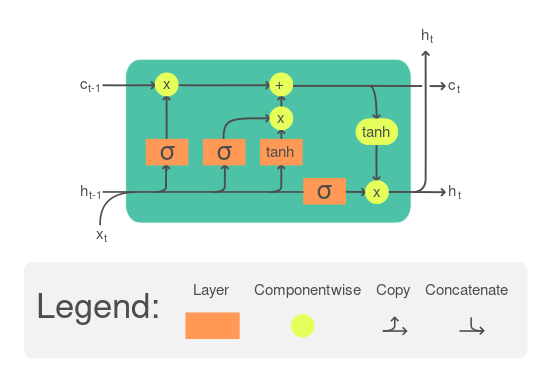
\includegraphics[width=0.7\linewidth]{assets/LSTM_Cell.png}
        \caption{LSTM memory cell}
        \label{fig:lstm-memory-cell}
    \end{figure}
    In \autoref{fig:lstm-memory-cell}, $x_t$ is the input vector, $h_t$ is the hidden state vector and $c_t$ is the cell state vector. Each of the layers in the figure's legend or gates have a feedforward network architecture with its weights and biases. The forget gate decides what information to discard from the previous state, the input gate decides which pieces of new information to store in the current cell state and the output gate controls which pieces of information in the current cell state to output. The cell state remembers values over arbitrary time intervals. Over training, the parameters of the different gates are adjusted. 

    LSTM networks can thus retain temporal relationships over arbitrary lengths. They were developed in \cite{hochreiter_schmidhuber_1997} as an alternative to Recurrent Neural Networks (RNN). These are a simpler NN architecture designed to handle sequential data, which through a series of feedback connections are allowed to retain information about previous states. RNN however have some computational issues commonly referred to as the vanishing gradient problem which prevents them from learning after a certain point. This issue is solved through the LSTM architecture. It also has some other quite useful characteristics such as also being able to model complex non linear relationships with more freedom than other classical ML models and can also provide multi step forecasting, allowing for modeling of a certain period in less steps. 

    The input vector again contains lags of the modeled series and the other two series as well as fourier decomposition components. 

    The main issue with LSTM is however its much higher computational complexity compared with simpler models, as well as needing large amounts of data and being more prone to overfitting than other simpler models. 
    
    \item \textbf{N-BEATS}: The Neural Basis Expansion Analysis for interpretable Time Series forecasting is another relatively new NN architecture focused on time series modeling through deep learning, mainly on the univariate case. Its architecture can be summarized through the following diagram obtained from the mentioned paper:
    \begin{figure}[ht]
        \centering
        \captionsetup{justification=centering}
        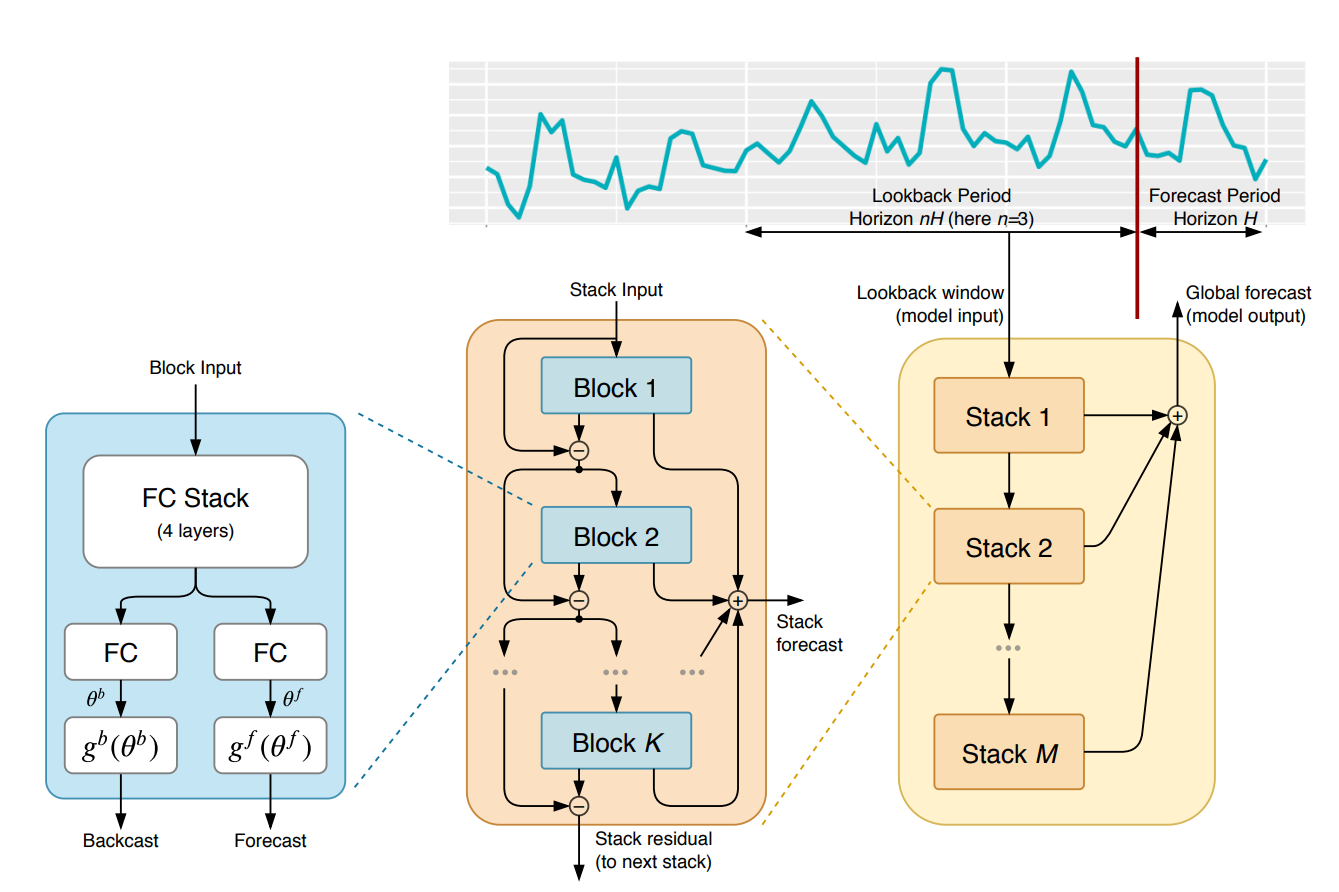
\includegraphics[width=\linewidth]{assets/nbeats-architecture.png}
        \caption{N-BEATS architecture}
        \label{fig:nbeats-architecture}
    \end{figure}
    Through \autoref{fig:nbeats-architecture} it can be seen how the model works. There are several stacks, each created by blocks of fully connected feedforward networks. Each block predicts a part of the forecast with the information from the lookback period. The fully connected stack in the block predicts both the forecast and the backcast -- data in the lookback period. The backcast is subtracted to the previously available lookback period, so each block tries to model the forecast from the residuals of the previous block in a very similar way to how each of the trees in the XGBoost predicts the error of the previous tree. The output of each of the blocks is summed to create the stack output, and all the stack's outputs is aggregated to create the final forecast. This architecture is supposed to automatically decompose the time series into different components like trend and seasonality in an interpretable way. This model has demonstrated state of the art performance in several time series benchmarks such as the M3 and M4. It is also domain agnostic, making no assumptions on stationarity or seasonality and it works well without any feature engineering. The training is also more efficient than for an LSTM, as the lack of recurrent feedback loops allows for parallelization of the training. It also allows for a multistep forecasting window. 
    
    \item \textbf{N-HiTS}: The Neural Hierarchical Interpolation for Time Series forecasting is another quite a recent architecture developed by \cite{challu_olivares_oreshkin_garza_2022}. It was developed with the explicit goal of modeling long term relationships in time series data in a more memory and computation efficient way. The architecture overview can be seen in the following diagram, obtained from the mentioned paper:
    \begin{figure}[ht]
        \centering
        \captionsetup{justification=centering}
        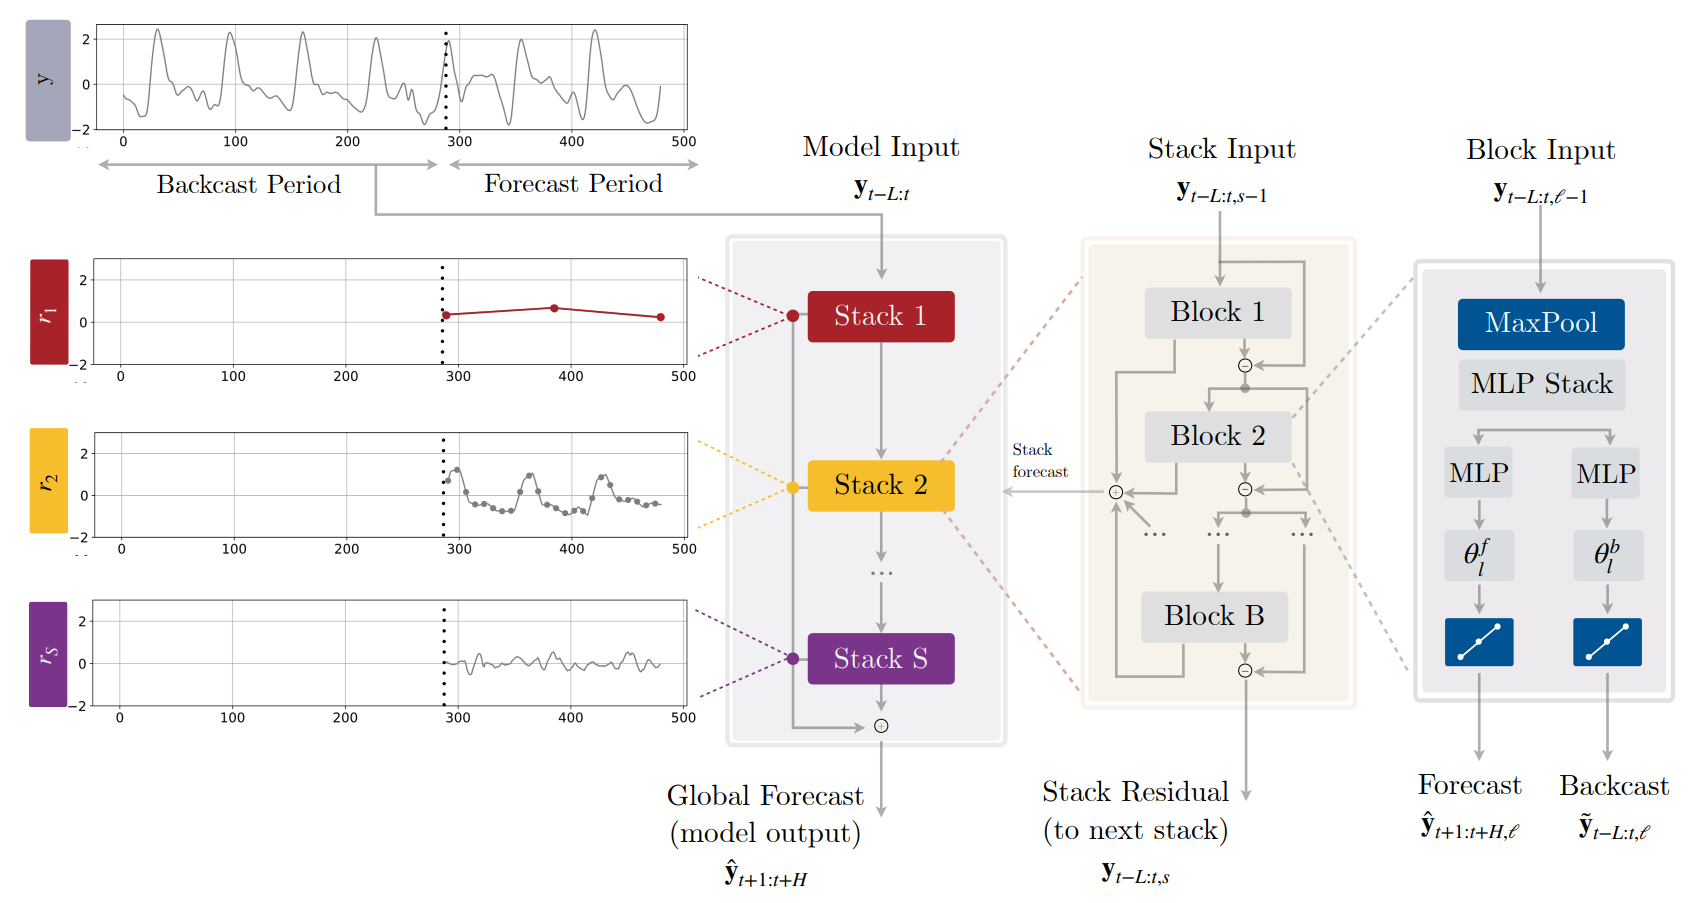
\includegraphics[width=\linewidth]{assets/nhits-architecture.png}
        \caption{N-HiTS architecture}
        \label{fig:nhits-architecture}
    \end{figure}
    As it can be seen in \autoref{fig:nhits-architecture}, the architecture is quite similar to the N-BEATS model with some added complexity. The model works first by sampling the historical window used in forecasting at different frequencies. Then, a series of MLP (feedforward NN) stacks are used in an ensemble way to forecast the following datapoint at each of the different forecasting frequencies. In the ensemble, each of the MLP stacks produces a prediction of the historic data which is substracted from the previous historic data, so each MLP block exclusively tries to approximate the residuals of the previous one -- very similarly to how each tree reduced the error of the previous tree in the XGBoost model. Then, the predictions across all frequencies are interpolated to provide a prediction for each of the minimal frequency datapoints. 
    
    This architecture allows each stack to focus on capturing the relationships at a different frequency, and it does it in a very efficient way, not really needing all datapoints for all relationships. This allows for very good performance in several long term time series as shown in the mentioned paper. Even if this is exclusively an univariate model, it has been shown to outperform several state of the art multivariate models. It remains to be seen however if following an exclusively univariate effect the cross relationships between all three series can be maintained.
    
    Also note how given the architecture, in this case it is not necessary to explicitly include time related variables such as the fourier decompositions as inputs, as these relationships are automatically learnt through the different frequencies' sampling.
\end{itemize}
\subsubsection{Transformer models}
Transformers are in reality also a type of deep learning or NN model. However it incorporates a series of new key components that make it different enough to merit its own category. Introduced by \cite{vaswani_2017} in the legendary \textit{Attention is All You Need} paper that sparked the LLM revolution, the transformer architecture is a NN architecture that incorporates a self-attention mechanism used to process traditional data. This self-attention mechanism is in simple terms a way of weighting the importance of different elements in a sequence relative to each other. This allows for a weighted sum of the input sequence focusing on relevant past information. It also contains other key components like the Positional Encoding, which is added to the input sequence to provide information about the position of each element in the such sequence. This general architecture is immensely flexible and has been applied successfully to many different problems, most notably to natural language generation. This basic model has also sparked a series of subsequent models with some modifications that make them specially suited for some tasks such as time series modeling. The architectures used in this work are:
\begin{itemize}
    \item \textbf{TFT}: Temporal Fusion Transformers introduced by \cite{lim_arık_loeff_pfister_2021} are a specific implementation of the transformer architecture used for time series modeling. It has three main components. The first is a set of Variable Selection Networks (VSN) which select the most relevant input variables. These can be static variables, dynamic historically known variables or dynamic generally known variables -- where not only the past values are known but future values are also known. The selected input goes into an LSTM based encoder which captures short term dependencies. Finally, a self-attention based decoder captures long term dependencies using transformers. All of this is coordinated through different gating mechanisms that modulate the flow of information between the different layers. A final key feature of this architecture is its in built ability to produce quantile forecasts. This however will not be specially useful for the task at hand. A more in depth overview of the architecture can be seen in \autoref{fig:tft-architecture}, obtained from the aforementioned paper. 
    \begin{figure}[ht]
        \centering
        \captionsetup{justification=centering}
        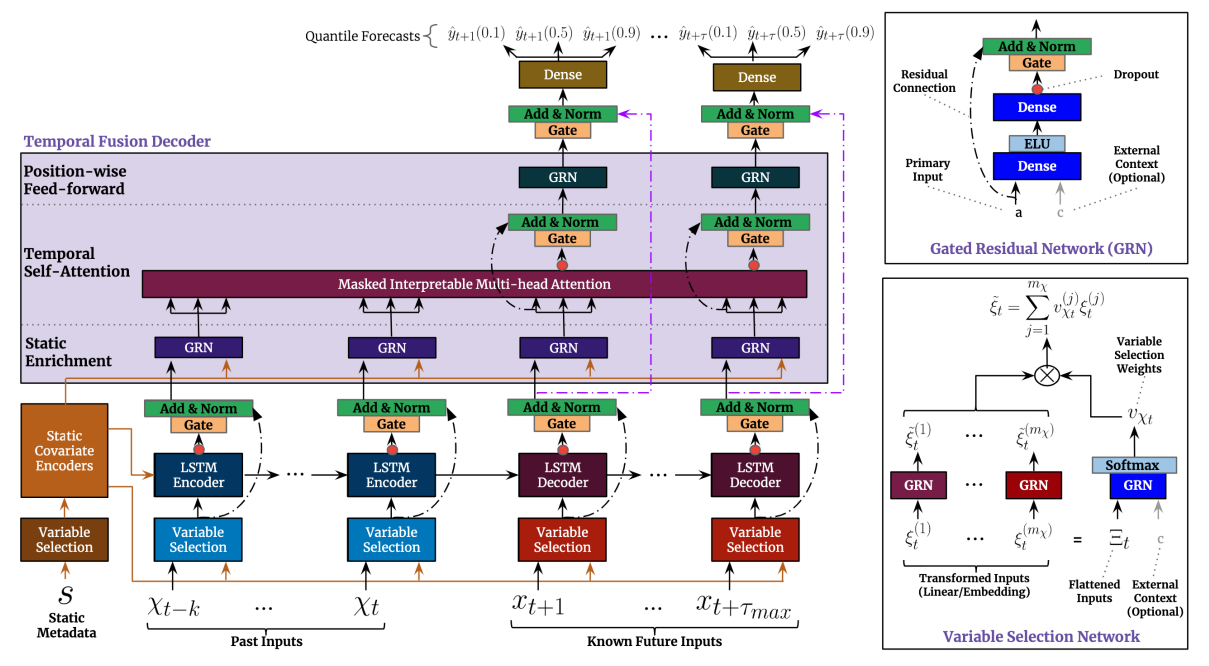
\includegraphics[width=\linewidth]{assets/tft-architecture.png}
        \caption{TFT architecture}
        \label{fig:tft-architecture}
    \end{figure}
    The TFT architecture has some very interesting features like explicitly capturing short and long term dependencies, regularization through the gating mechanisms, multi step prediction or interpretability of variable importance. However this comes at the expense of high computational cost, high model complexity and high data requirements.
    \item \textbf{Informer}: A different transformer based architecture developed by \cite{zhou_zhang_peng_zhang_li_xiong_zhang_2021} specifically developed for forecasting of long sequence time-series through a more efficient implementation. The main advances introduced in this model are the use of a \textit{ProbSparse} self-attention mechanism which has a time and memory complexity of $\mathcal{O}(n\log n)$ instead of $\mathcal{O}\left(n^2\right)$ -- with $n$ being the lookback period --, a decoder which predicts the long time-series sequence in one operation rather than step by step and an input method specifically developed to handle extremely long input sequences. 
    
    The Informer has many of the same benefits of other transformer based architectures, but with the added feature of being more efficient and thus being able to incorporate a longer lookback period and thus capturing longer range dependencies that may escape some other architectures. All the while being also more efficient at inference time and thus faster in formulating predictions. However, it also shares many of the same disadvantages of other transformer based models like requiring vast amounts of data for proper training or being very resource intensive, even with the added efficiency.  
    \item \textbf{FEDFormer}: The Frequency Enhanced Decomposed Transformer presented by \cite{zhou_ma_wen_wang_sun_jin_2022} is yet another transformer based architecture specially designed for long sequence time series modeling. It leverages a principle similar to the N-HiTS. It uses the idea that complex time series have a much more compact representation in the frequency domain, which also captures both long term trends and shorter term seasonal components. To act upon this principle, the authors make several changes to the base transformer architecture, substituting the Multi-Headed Self-Attention block with a Frequency Enhanced Block and the Multi-Headed Cross-Attention block with a Frequency Enhanced Attention block. Both of these leverage Fourier transforms within their operations to operate on the frequency domain. However, the authors also provide the option of using the Wavelet Transform (WT) instead of the Fourier Transform (FT). Using the WT which transforms the input to the frequency and time domain, not only to the frequency domain as the FT, allows for a more nuanced although complex representation of the input data. For this work, the FT implementation will be used due to its simpler implementation. 
    
    Altering the transformer to operate on the frequency domain also has as a consequence reducing the complexity further down even from the Informer to linear time and memory. 
    
    Appart from accentuating the benefits already mentioned in the Informer, in the paper it is demonstrated how the predicted distribution is closer to the ground truth distribution according to the Kolmogorov-Smirnov distribution test, which is a specially interesting characteristic given the work objectives and evaluation metrics explained in \autoref{s:evaluation-metrics}.

    \item \textbf{iTransformer}: \textcolor{red}{COMPLETE SECTION}
\end{itemize}
\subsubsection{Comparison}
After having presented all model classes and the different models that will be implemented themselves, it can be useful to perform a quick comparison and an a priori judgement of which models should outperform the rest, even if all of them will be implemented and evaluated. 

It can be seen how there is a very wide range of models from which to chose from -- many more than the ones presented here. It is worth noting how here only the base models have been analyzed, and no custom combinations between them have been explored. These combinations can be very useful in combining useful characteristics of two or more base models and creating more accurate predictions as shown in \cite{zou_yang_2004}.

Out of all models here analyzed, it would seem like the most appropriate due to its intrinsic characteristics is the FEDFormer due to it being able to include a very long forecasting horizon and lookback periodin each step, combined with a reasonable robustness that allows it to maintain the capacity to learn long run complex patterns.

All of these characteristics are also shared to a greater or lesser extent by the N-BEATS and N-HiTS, but the FEDFormer can be deployed in a multivariate setup, while N-HiTS and N-BEATS are exclusively univariate. This would force to include the information of the other series as exogenous variables, while a multivariate approach is more straightforward and potentially with less accumulated error for multi step ahead predictions.  

The FEDFormer also allows for the use of specific loss functions that could be used to improve accuracy in extreme values. 
% Roughly it can be seen how the different models can be placed along a complexity axis, from the classical statistical ones being the most simple and the transformer based ones being the most complex. In this complexity axis one can find high interpretability, robustness to overfitting, efficiency and ease of training and prediction on the simple end and capability to learn complex long run patterns, predict multiple steps ahead in one run

\subsection{Loss functions}
\label{s:loss-functions}
As previously mentioned, one of the main concerns with long horizon models used to predict solar and wind generation -- even more so in the case of wind -- is its ability to accurately model the extreme values of the generation distribution. The reasoning for this was already explained in  subsection \nameref{s:modeling-task-characteristics}. 

One way of enabling models to better approximate these values is through the loss function used to train them. The loss function is a mathematical function that measures how well a model's predictions align with the actual values. It quantifies the errors of the model and guides the learning process, as the model will try to minimize this loss function. Some commonly used loss functions are the Root Mean Squared Error, the Mean Absolute Error or the Kullback-Leibler Divergence for example. The choice of the loss function guides the finally optimal model and thus its performance. A possibility that will be tested in this work is whether modifying the standard loss function to one that penalizes more heavily errors in the extremes can lead to a model with better performance in extreme value metrics. The loss function that will be used for this is the Squared Error Relevance Area introduced in \cite{silva_ribeiro_moniz_2022}.
\subsubsection{SERA}
The Squared Error Relevance Function is a loss function that tries to give a bigger emphasis to errors commited in the extremes while still accounting for the performance in the rest of the distribution, thus preventing a severe bias from occurring. 

Given a set of points $\mathcal{D}=\{\langle x_i,y_i\rangle\}^N_{i=1}$ and a relevance function $\phi :\mathcal{Y} \rightarrow \{0,1\}$ defined for the target variable $Y$. Consider the subset $\mathcal{D}^t\subseteq \mathcal{D}$ defined as $\mathcal{D}^t=\{\langle x_i, y_i\rangle \in \mathcal{D} | \phi(y_i)\geq t\}$ the Squared Error Relevance with respect to a given cutoff $t$ $(SER_t)$ is defined as 
\begin{equation}
    SER_t=\sum_{y_i \in \mathcal{D}^t}(\hat{y}_i-y_i)^2
\end{equation}
By integrating this function overa all $t$ the $SERA$ is obtained
\begin{equation}
    SERA=\int_0^1 SER_t dt
\end{equation}

In this case the relevance function $\phi(\cdot)$ is heavily inspired on the one used in the referenced paper. It is a Cubic Hermite spline. This is a curve where each segment is a third order polynomial specified by the value and first order derivative at each of the end points. Two intermediate points are chosen according to upper and lower chosen percentiles. For example, the $y$ values for the 10th and 90th percentile values are chosen. These values will be $x$ values for the $\phi(\cdot)$ function with a 0 first degree derivative and 0 or 1 $y$ value, depending on whether the $SERA$ function has been specified to focus on the lower or upper extreme values. If the the model is to focus on the upper extreme values, the 90th percentile will have a $y$ value of 1 and the 10th a value of 0. Furthermore, the 0 and 1 points -- as these are the theoretical minimum and maximum values for the capacity factor -- are determined to have a 0 derivative and a 1 or 0 $y$ value, again depending on whether this is the upper or lower $SERA$. 

Note how many of the models mentioned in the \nameref{s:models} section are able to work with custom loss functions. However, to analyze whether a custom loss function helps in improving model accuracy for extreme values it is not necessary to retrain all models with this loss function. A single model will be trained with this loss function and its results will be compared to those obtained with the baseline loss function (MAE). The chosen model for the analysis has been the XGBoost given its ease of training and simplicity. In order to implement the $SERA$ loss function for the XGBoost library, functions defining its gradient and hessian have been created.
\subsection{Evaluation metrics}
\label{s:evaluation-metrics}
\textcolor{red}{REWRITE METRICS AFTER IMPLEMENTATION WHERE NECESSARY}
In order to understand why the following metrics have been chosen for evaluation it is important to keep in mind the overarching goal of the project. The goal of the mentioned models is not to provide an accurate short term forecast, but to provide a model that porperly simulates the long term dynamics of the three time series. That is, models that are able of producing long term scenarios of solar and wind generation with univariate and multivariate dynamics equivalent to the real world ones, in order to optimize and test several grid planning possiblities on these scenarios. 

In order to best achieve this goal, the best performing model will have to be evaluated on different metrics, each corresponding to different attributes needed for correct whole picture modeling. These are the different attributes that will be tested and the metrics that will be used to test them. 

\subsubsection{Marginal distributions}
The first metric that will be evaluated will be the similarity of the univariate series with the real world data. Note that this similarity is not a pointwise similarity. In many relevant papers, the accuracy of a series predicition is calculated through metrics like the RMSE or the MAPE. However, these metrics require that the prediction try to get right the value at each timestep. If there is a delay of one timestep, or a "cloudy week" comes a week earlier or later the RMSE will give a very poor score even though the general behaviour is the same. That is why the approach taken here will be slightly different. The metrics used will be the following:
\begin{itemize}
    \item \textbf{Cramér von Mises criterion}: The Cramér von Mises criterion intriduced by \cite{cramer_28} measures the distance between two CDF. It is calculated like:
    \begin{equation}
        \omega^2=\int_{-\infty}^{\infty}\left[F_m\left(x\right)-F_e\left(x\right)\right]^2dF_e\left(x\right)
    \end{equation}
    Where $F_m\left(x\right)$ is the modelled empirical CDF and $F_e\left(x\right)$ is the observed empirical CDF.
    \item \textbf{Kullback-Leibler divergence}: The KL divergence or relative entropy introduced in \cite{kullback_leibler_1951} is a statistical distance that measures how different a probability distribution is from another reference one. It is calculated like
    \begin{equation}
        D_{KL}\left(P||Q\right)=\sum_x P\left(x\right)\log{\left(\frac{P\left(x\right)}{Q\left(x\right)}\right)}
    \end{equation}
    where $P$ is the modelled probability distribution and Q is the reference probability distribution.
    \item \textbf{ACF distance}: Even though the marginal distributions are by themselves a fundamental part of the closeness of the univariate series to reality, they are not the only one. Another key aspect of the series is its termporal self dependency, studied through the ACF of the correlation coefficient and the new correlation coefficient in the section called \nameref{sec:lagged-relationships}. The difference between the ACF of the $\xi$ metric of the empirical data and the model will be measured through a weighted root mean squared error, calculated as:
    \begin{equation}
        \text{ACFD}=\sqrt{\frac{\sum_{k=0}^N |w_k|\left[ACF_m\left(k\right)-ACF_e\left(k\right)\right]^2}{\sum_{k=0}^N |w_k|}}
    \end{equation}
    where $N$ is the number of periods for which the metric is calculated -- 72 in this case, $ACF_m$ is the model's $\xi$ ACF, $ACF_e$ is the empirical $\xi$ ACF and $w$ is the weighting factor, determined to be $w_k=ACF_e\left(k\right)$. This has been chosen so a higher weight is given to those lags with a higher empirical relevance. 
    % \item \textbf{Seasonal metrics}: The metrics above will be calculated on the overall sample but also on subsamples divided by yearly season and daily period, to ensure the fit not only on a global scale but also on specific periods. 
\end{itemize}
\subsubsection{Joint distributions}
Now that it is clear how the marginal distributions will be assessed, it is time to look at how the dependence structure between the three series will be tested. There are several metrics that will be used for that purpose:
\begin{itemize}
    \item \textbf{Copula correlation matrix distance}: In the section regarding \nameref{sec:multivariate-analysis}, the correlation matrix of a gaussian copula representing the dependence structure between the series was calculated. The same matrix will be calculated for samples of each of the models. Then, the distance (CCMD) between both matrices will be calculated. This distance is calculated as:
    \begin{equation}
        CCMD=\sqrt{\sum_i\sum_j\left(a_{ij}-b_{ij}\right)^2}
    \end{equation}
    where $A=\{a_{ij}\}$ is the correlation matrix of the copula fitted to the modelled data and $B=\{b_{ij}\}$ is the correlation matrix shown in \autoref{table:copula-correlation-matrix}.
    \item \textbf{CCF distance}: The cross correlation function distance is analogous to the autocorrelation function distance explained above, but for the $\xi$ cross correlation function instead of ACF.
    % \item \textbf{Seasonal metrics}: Similarly to the univariate case, the metrics above will be calculated on the whole period but also with seasonal differences and daily period differences.
\end{itemize}

\subsubsection{Extreme value analysis}
A significantly important aspect of the models is their need to be particularly accurate on the extreme values. Periods of extreme wind or solar generation are particularly interesting to the grid, due to their displacement of other energy sources or their need of them. That is why the accuracy of the models on extreme values will be assessed through these metrics:
\begin{itemize}
    % \item \textbf{Anderson-Darling statistic}:
    \item \textbf{Conditional Value at Risk}: The CVaR, usually used in financial risk management, measures what a certain value on average will be given that a certain threshold has been exceeded. It is calculated as 
    \begin{equation}
        \text{CVaR}_{\alpha}(x) = \mathbb{E} \left[X\mid X>\text{VaR}_{\alpha}\right]
    \end{equation} 
    with $\text{VaR}_{\alpha}$ being the Value at Risk for a given certainty. That is, the maximum value not exceeded with a probability $\alpha$. It is characterized as 
    \begin{equation}
        \text{VaR}_{\alpha}=\text{inf}\{x|F_X(x)\geq\alpha\}
    \end{equation}
    The assessment metric will be the difference between the CVaR calculated as 
    \begin{equation}
        \text{CVRD}=\frac{\text{CVaR}^m_{95\%}}{\text{CVaR}^e_{95\%}}-1
    \end{equation}
    where $\text{CVaR}^m_{95\%}$ is the CVaR at a 95\% level for the model and $\text{CVaR}^e_{95\%}$ is the empirical CVaR at a 95\% level.
    \item \textbf{Tail dependence}: The tail dependence coefficient is a measure of the comovements of the tails of their distributions. It can be lower tail dependence or upper tail dependence, with the lower tail dependence calculated as 
    \begin{equation}
        \lambda_l=\lim_{q \to 0} P\left(X_m \leq F^{-1}_m(q) \mid X_e \leq F^{-1}_e(q)\right)  
    \end{equation}
    and the upper tail dependence coefficient being calculated as 
    \begin{equation}
        \lambda_u=\lim_{q \to 1} P\left(X_m > F^{-1}_m(q) \mid X_e > F^{-1}_e(q)\right)  
    \end{equation}
    with $F^{-1}_m$ being the inverse CDF for the model and $F^{-1}_e$ being the empirical inverse CDF.

    There will be two comparisons. The comparison of the tail dependence between each pair of modeled variables with that of the corresponding pair of empirical variables -- e.g. tail dependence between modeled solar PV and modeled wind and tail dependence between empirical solar PV and empirical wind -- and also the tail dependence between each modeled variable with its corresponding empirical varaiable -- e.g. tail dependence between modeled solar PV with empirical solar PV.  
    \item \textbf{Return level}: The GEV function is a function often used to model the maxima of sequences of random variables. Its CDF is
    \begin{equation}
        P\left(GEV\left(\mu,\sigma,\xi\right)\leq x\right)=e^{-t\left(x\right)}
    \end{equation}
    with
    \begin{equation}
        t\left(x\right)\equiv 
        \begin{cases} 
        \left[ 1 + \xi \left( \frac{x - \mu}{\sigma} \right) \right]^{- \frac{1}{\xi}}, & \text{if } \xi \neq 0, \\
        e^{\left( - \frac{x - \mu}{\sigma} \right)}, & \text{if } \xi = 0.
        \end{cases}
    \end{equation}
    As it can be seen from the formulation above the distribution of maximum values depends on three variables, with $\xi$ governing the tail behaviour. Once the GEV distribution is fitted to the data, the return level can be estimated. The return level is the value expected to be exceeded on average once in a given period. If the 100 year return level of wind capacity factor is 0.95, that means that on average there will be one instance every 100 years where the capacity factor exceeds 0.95. The return level $z_T$ is calcualted as 
    \begin{equation}
        z_T=\mu+\frac{\sigma}{\xi}\left[\left(-\text{log}\left(1-\frac{1}{T}\right)\right)^{-\xi}-1\right]
    \end{equation}
    Thus, the weekly maxima will be obtained with the data, with which a GEV distribution will be fitted and a 10 year return level will be calculated. The assessment metric will be the percentage difference in return level calculated as 
    \begin{equation}
        \text{RLD}=\frac{z^m_{10}}{z^e_{10}}-1
    \end{equation}
    This will be calculated for both the maxima and the minima of the distributions. 
\end{itemize}

The extreme value assessment is particularly important for wind generation, rather than for solar generation as it is much more consistent. Therefore, these values will only be calculated for the wind series. 

\subsection{Model training and validation}
After having layed out the different evaluation metrics that will be used, the method used for training and validating the models will be presented. 

A general train-test-validation split will be used. This approach splits the available data in three groups. The first will be used to train the models. The second will be used to test the models and iteratively improve these models, by checking for overfitting and evaluating different parameter setups. The validation data is left as a the final evaluation data, where the final metrics that will be presented are calculated. The metrics obtained in this group can be seen as the metrics that are to be expected of the models in a real world context after deployment. A split of 1 year validation data, 1 year testing data and the rest as training data has been chosen, as a 1 year prediction horizon is a long enough horizon to test the long run characteristics of the model and it contains values for all different seasons. 

As it can be seen in the \nameref{s:evaluation-metrics} section there are many different evaluation metrics attempting to check for different characteristics of the model. Therefore, using a programatic approach to model creating through something like a gridsearch of parameters is not really useful, as it can be difficult to determine in an algorithmic way which results are better than others, as one model can have better results modeling extreme values while other can have better results in modeling cross relationships. Therefore, a manual approach to model improvement with the test set will be employed, and only the best overall model selected in a discretionary way will be evaluated on the validation set and will have its results presented in this work.

Another thing worth mentioning is that no cross validation or bootstrapping methods will be used to evaluate the models. Although these approaches would give a more robust understanding of the validity of the model by being more resistant to anomalies in the test and validation sets, the amount of data available for training -- specially for the neural network and transformer based models -- is not enough in order to sacrifice even more for testing and validation purposes.

As an alternative approach to cross validation and bootstrapping, the test and validation sets will be evaluated for anomalies. That is, they will be evaluated as if they were a prediction against the previous year. The results are the following:

\begin{table}[ht]
    \centering
    \begin{tabular}{rll}
        \toprule
        Solar PV & \multicolumn{2}{c}{Period} \\ 
        \cmidrule(lr){2-3}
            & Test & Validation \\
        \midrule
        Cramer von Mises & 29.34 & 9.48 \\
        KL divergence & 0.0003 & 0.0004 \\
        ACF$_\xi$ distance & 0.0127 & 0.0137 \\
        \midrule
        CCMD & 0.0112 & 0.0167 \\
        CCF$_\xi^{Solar TH}$ distance & 0.0099 & 0.0338\\
        CCF$_\xi^{Wind}$ distance & 0.0119 & 0.0372 \\
        \midrule
        CVaR$^+$ distance & -0.0297 & -0.0064 \\
        % CVaR$^-$ distance & 0.8416 & -0.2067 \\
        Tail dependence coefficient$^+$ & 0.3676 & 0.4703 \\
        % Tail dependence coefficient$^-$ & 0.1119 & 0.1381 \\
        Return level distance$^+$ & 0.0154 & -0.0248 \\
        % Return level distance$^-$ & 0.0289 & -0.0661 \\
        \bottomrule
    \end{tabular}
    \caption{Evaluation metrics of the test and validation sets with respect to the previous year for solar PV}
    \label{table:eval-metrics-test-validation-solar-pv}
\end{table}

At a first glance it can be seen how some metrics seem to be more consistent than others. The Cramer von Mises statistic for example exhibits what seems to be a great difference between one and the other year, while the KL divergence seems to be more reliable exhibiting a much lesser difference. These values will be useful as they represent a baseline of what a reasonable \textit{error} according to the different metrics would be. If when evaluating a model the metric is similar to the ones shown here, the predicted values can be approximated to be close enough to what a the real process would generate. 

Note how for solar PV the metrics regarding the extreme values in the left tail have been left out, as the values here are very close to zero and thus these metrics are very noisy. The same will be done for solar TH. 

\begin{table}[ht]
    \centering
    \begin{tabular}{rll}
        \toprule
        Solar TH & \multicolumn{2}{c}{Period} \\ 
        \cmidrule(lr){2-3}
            & Test & Validation \\
        \midrule
        Cramer von Mises & 12.86 & 9.89 \\
        KL divergence & 0.0102 & 0.0265 \\
        ACF$_\xi$ distance & 0.0249 & 0.0162 \\
        \midrule
        CCMD & 0.0112 & 0.0167 \\
        CCF$_\xi^{Solar PV}$ distance & 0.0151 & 0.0155 \\
        CCF$_\xi^{Wind}$ distance & 0.0201 & 0.0229 \\
        \midrule
        CVaR$^+$ distance & 0.0732 & -0.1318 \\
        % CVaR$^-$ distance & 0.8416 & -0.2067 \\
        Tail dependence coefficient$^+$ & 0.3356 & 0.2968 \\
        % Tail dependence coefficient$^-$ & 0.1119 & 0.1381 \\
        Return level distance$^+$ & 0.2928 & -0.1504 \\
        % Return level distance$^-$ & 0.0289 & -0.0661 \\
        \bottomrule
    \end{tabular}
    \caption{Evaluation metrics of the test and validation sets with respect to the previous year for solar TH}
    \label{table:eval-metrics-test-validation-solar-th}
\end{table}

In \autoref{table:eval-metrics-test-validation-solar-th} the same metrics shown before but for solar TH can be seen. Again, these will be used as benchmarks for the modeling of solar thermal by the different models. Note how the CCMD metrics are the same, as the copula matrix is the same one for all three series, and the distance is thus also equivalent.

\begin{table}[ht]
    \centering
    \begin{tabular}{rll}
        \toprule
        Wind & \multicolumn{2}{c}{Period} \\ 
        \cmidrule(lr){2-3}
            & Test & Validation \\
        \midrule
        Cramer von Mises & 9.48 & 5.01 \\
        KL divergence & 0.0.0018 & 0.0018 \\
        ACF$_\xi$ distance & 0.0602 & 0.0630 \\
        \midrule
        CCMD & 0.0112 & 0.0167 \\
        CCF$_\xi^{Solar PV}$ distance & 0.0128 & 0.0111 \\
        CCF$_\xi^{Solar TH}$ distance & 0.0136 & 0.0131 \\
        \midrule
        CVaR$^+$ distance & -0.0236 & -0.0016 \\
        CVaR$^-$ distance & -0.2461 & 0.2123 \\
        Tail dependence coefficient$^+$ & 0.0479 & 0.2443 \\
        Tail dependence coefficient$^-$ & 0.1506 & 0.1119 \\
        Return level distance$^+$ & 1.3618 & -0.0071 \\
        Return level distance$^-$ & -13.5111 & -1.1904 \\
        \bottomrule
    \end{tabular}
    \caption{Evaluation metrics of the test and validation sets with respect to the previous year for wind}
    \label{table:eval-metrics-test-validation-wind}
\end{table}

Finally in \autoref{table:eval-metrics-test-validation-wind} the same metrics that will be used as benchmarks for wind can be seen. Here, the metrics relating to the extremes in the negative tail have been included since for wind it does hold some interest to see whether the model accurately models periods of low wind generation.
\newpage
\section{Results}
After having described all the different implemented models, having formulated a hypothesis about which should be able to outperformed and explained how the models are trained and evaluated, it is now time to present and analyze the obtained results. This section will have four subsection. The first three will focus on each of the three capacity factors, analyzing separately which models outperform and why in each of them. The final section will be devoted to analyzing whether the custom loss function successfully outperforms the base loss function in extreme value modeling. 
\subsection{Solar PV}
\label{s:solar-pv-results}
The first results that will be presented are those of the photovoltaic solar capacity factor. The results will be presented for all metrics for all evaluated models in a similar way as was presented in \autoref{table:eval-metrics-test-validation-solar-th}: \nameref{table:eval-metrics-test-validation-solar-th}.

The metrics of the validation set obtained in the \nameref{s:model-training-and-validation} section will also be included as a reference point. 
\newpage
\begin{table}[ht]
    \footnotesize
    \begin{tabular}[l]{r|c|ccc|cc|}
        \toprule
        \textbf{Solar PV} &Benchmark&Regression&SARIMAX&VARMAX&SVM&XGBoost \\ 
        \midrule            
        Cramer von Mises&29.34&364.6&93.27&295.7&223.3&747.4 \\
        KL divergence&0.0002762&0.4844&0.1905&1.692&0.1662&1.586 \\
        ACF$_\xi$ distance&0.0127&0.1201&0.1089&0.1163&0.2289&0.1802 \\
        \midrule
        CCMD&0.01117&0.3291&0.1044&0.2151&0.8375&0.3549 \\
        CCF$_\xi^{Solar TH}$ distance&0.009855&0.1232&0.08045&0.223&0.1484&0.3242 \\
        CCF$_\xi^{Wind}$ distance&0.01187&0.07759&0.04984&0.1515&0.1091&0.8558 \\
        \midrule
        CVaR$^+$ distance&-0.02966&8.394&0.08376&-0.6706&0.6503&-0.7125 \\
        Tail dependence coefficient$^+$&0.3676&0.2671&0.3174&0.000&0.1187&0.03397 \\
        Return level distance$^+$&0.01537&1.857e+07&-0.3411&-1.091&0.7803&-0.9312 \\
        \bottomrule
    \end{tabular}
\end{table}
\begin{table}[ht]
    \footnotesize
    \begin{flushright}
    \begin{tabular}[r]{|ccc|cccc}
        \toprule
        N-BEATS&N-HiTS&TimeMixer&TFT&Informer&FEDFormer&iTransformer  \\
        \midrule            
        69.43&47.81&52.58&2221&485.8&158.6&131.1 \\
        0.3452&0.003905&0.04968&2.721&1.302&0.5261&0.01814 \\
        0.1018&0.06985&0.04528&0.1769&0.2429&0.1729&0.05605 \\
        \midrule
        0.1959&0.4296&0.05632&0.5398&0.5675&0.5183&0.2093 \\
        0.0481&0.1829&0.0826&0.2603&0.1649&0.2608&0.0688 \\
        0.02316&0.01634&0.07532&0.4126&0.06594&0.1383&0.08443 \\
        \midrule
        1.037&0.003395&0.1888&-0.9442&-0.6828&-0.3569&0.1683 \\
        0.2831&0.3265&0.2032&0.000&0.04338&0.002283&0.3699 \\
        4.802&-0.1408&0.7089&-1.09&-0.02178&-0.3841&0.2181 \\
        \bottomrule
    \end{tabular}
    \end{flushright}
    \caption{Results of the different models for Solar PV\label{long}}
    \label{table:results-solar-pv}
\end{table}
Given the great number of metrics and the difficulty of easily interpreting them, here is another table with the rank of the model for each metric. That is, for each metric, each model will be shown as the 1st, 2nd, 3rd... best model. The benchmark has also been included in this ranking. In most metrics a lower value is better, while for the distances in the extreme values category it is having a lower absolute value what is important, as the deviation in either sense is negative. The Tail dependence coefficient is the only metric where a higher value is better. In bold, the best model -- apart from the benchmark -- is highlighted. 
\newpage
\begin{table}[ht]
    \footnotesize
    \begin{tabular}[l]{r|c|ccc|cc|}
        \toprule
        \textbf{Solar PV} &Benchmark&Regression&SARIMAX&VARMAX&SVM&XGBoost \\
        \midrule            
        Cramer von Mises&(1)&(10)&(5)&(9)&(8)&(12) \\
        KL divergence&(1)&(8)&(6)&(12)&(5)&(11) \\
        ACF$_\xi$ distance&(1)&(8)&(6)&(7)&(12)&(11) \\
        \midrule
        CCMD&(1)&(7)&(3)&(6)&(13)&(8) \\
        CCF$_\xi^{Solar TH}$ distance&(1)&(6)&(4)&(10)&(7)&(13) \\
        CCF$_\xi^{Wind}$ distance&(1)&(7)&(4)&(11)&(9)&(13) \\
        \midrule
        CVaR$^+$ distance&(2)&(13)&(3)&(8)&(7)&(10) \\
        Tail dependence coefficient$^+$&(2)&(6)&(4)&(12)&(8)&(10) \\
        Return level distance$^+$&(1)&(13)&(5)&(11)&(8)&(9) \\
        \bottomrule
        Total&(11)&(78)&(40)&(86)&(77)&(97) \\
        \bottomrule
    \end{tabular}
\end{table}
\begin{table}[ht]
    \footnotesize
    \begin{flushright}
    \begin{tabular}[r]{|ccc|cccc}
        \toprule
        N-BEATS&N-HiTS&TimeMixer&TFT&Informer&FEDFormer&iTransformer \\
        \midrule            
        (4)&\textbf{(2)}&(3)&(13)&(11)&(7)&(6) \\
        (7)&\textbf{(2)}&(4)&(13)&(10)&(9)&(3) \\
        (5)&(4)&\textbf{(2)}&(10)&(13)&(9)&(3) \\
        \midrule
        (4)&(9)&\textbf{(2)}&(11)&(12)&(10)&(5) \\
        \textbf{(2)}&(9)&(5)&(11)&(8)&(12)&(3) \\
        (3)&\textbf{(2)}&(6)&(12)&(5)&(10)&(8) \\
        \midrule
        (12)&\textbf{(1)}&(5)&(11)&(9)&(6)&(4) \\
        (5)&(3)&(7)&(12)&(9)&(11)&\textbf{(1)} \\
        (12)&(3)&(7)&(10)&\textbf{(2)}&(6)&(4) \\
        \bottomrule
        (54)&\textbf{(35)}&(41)&(104)&(79)&(80)&(37) \\
        \bottomrule
    \end{tabular}
    \end{flushright}
    \caption{Results of the rank of the different models for Solar PV\label{long}}
    \label{table:results-rank-solar-pv}
\end{table}

At the bottom of \autoref{table:results-rank-solar-pv} a Total can be found. This total is the sum of the rank of the model accross all metrics and it can be seen as a very simple proxy of the overall goodness of the model across all domains -- distribution fit, multivariate coherence and extreme value fit. 

%THIS WAS BEFORE CHANIGING RANK OF TAIL DEPENDENCE When first seeing these results many insights can be extracted. The first one is about the evaluation metrics themselves. By looking at \autoref{table:results-rank-solar-pv} one can see that the rank of a given model for the evaluation metrics in a given category -- distribution fit, multivariate coherence and extreme value fit -- are generally congruent with each other. That is, if one of the models is one of the best according to the Cramer von Mises metric for example, it will tend to be ranked highly also with the KL divergence and ACF$_\xi$ distance metrics. However, that is not the case for the Tail dependence coefficient$^+$. This metric can be more affected by temporal shifts in the extreme values than the other two, and thus it can be seen how it contains more noise than the others and does not reflect the same ranking among models. That is why, this metric will not be as highly taken into account as the other two extreme value metrics. However, it will still be included for completeness sake. 

The most relevant and straightforward insight that can be obtained from a quick glance at the results is the superiority of the NN based models in general, and more precisely of the N-HiTS model. This is most probably due to the high seasonality of the solar PV series. This model is speacially designed to operate at different frequencies, thus extracting all relevant frequency based patterns but without overfitting. When looking at each evaluation category, the N-HiTS seems to be the best regarding the general distribution of the forecast, while the TimeMixer seems to be somewhat better regarding the temporal self consistency -- that is, the how correlated a given value should be with its past values -- and the N-BEATS seems to be the better one regarding multivariate cross relationship. Finally in the extreme value modeling the N-HiTS again stands as the best model, with the other two NN models doing considerably worse. 

In the statistical methods a very big difference between the SARIMAX and the other two models can be seen. The SARIMAX is actually the best model after the N-HiTS and the iTransformer practically tying with the TimeMixer, performing quite well in all evaluation metric categories. This is again thanks to the SARIMAX being able to utilize the frequency components given by the fourier decompositions without overfitting. The order 1 integration in the SARIMAX however seems to be of critical importance, given how the other two statistical methods perform considerably worse and this is one of the main differences. 

Within the transformer based models there seems to also be a great difference between the iTransformer -- which is actually the second best model practically tied with the N-HiTS, doing worse in general distribution but better in multivariate coherence -- and the rest of the transformer models, with the latter being at a performance level similar to the vanilla Regression model. This could be attributed to the complexity of the models, which could have led them to overfitting. The good performance of the iTransformer with respect to the other architectures is consistent with the benchmarks performed by \cite{wang2024tssurvey}.  

Finally, regarding the machine learning methods the conclusions are similar to those of the transformer based models. Their performance is among the worst of all the models. They seem to have joined the worst characteristics of the simple statistical methods and the more complex NN based methods. The way of encoding seasonal and time varying data is not as sophisticated as for the NN models as they only use the Fourier decompositions, however by adding extra complexity in the way those decompositions are used compared to the statistical methods they seem to overfit and end up performing even worse than these simpler models. Among themselves, it seems like the SVM is better equiped than the XGBoost to model the solar PV data.

Here is a plot of the yearly and weekly for a random week modeled data, together with the actual data. Note how on a moment to moment basis the data does not need to be similar, as the goal is not to accurately predict the hourly value of the capacity factor, but to get a distribution of data with the same characteristics. 
\begin{figure}[ht]
    \centering
    \captionsetup{justification=centering}
    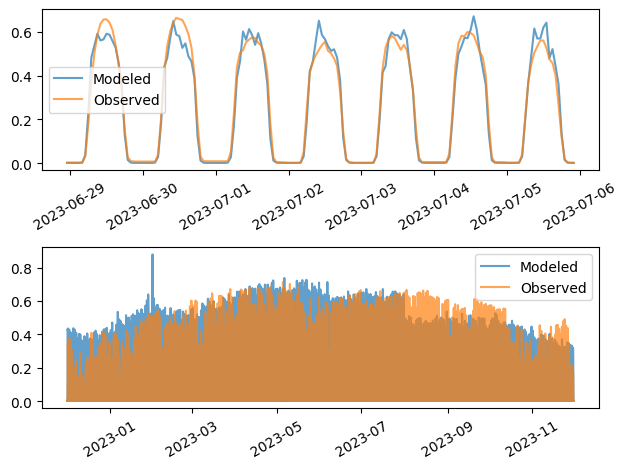
\includegraphics[width=0.7\linewidth]{assets/nhits-solar-pv.png}
    \caption{Weekly and yearly predicted and actual solar PV capacity factor for the N-HiTS model}
    \label{fig:nhits-solar-pv}
\end{figure}
Note how the modeled data is much more rugged on an hourly basis, while the actual data follows a much smoother hour to hour pattern. However, this model is still more accurate with that ruggedness than other smoother models like the SARIMAX or the VARMAX.  
On the yearly pattern it can be seen how the model greatly overestimates some extreme positive values and has some sudden drops in capacity factor around august, but the general patterns are maintained. 
\subsection{Solar TH}
For the solar thermal capacity factor series, the results will be shown in the same way as for the \nameref{s:solar-pv-results} section. The two tables showing the metrics' values and the rank of the models will be presented, and they will later be discussed. 

% \newpage
\begin{table}[ht]
    \footnotesize
    \begin{tabular}[l]{r|c|ccc|cc|}
        \toprule
        \textbf{Solar TH} &Benchmark&Regression&SARIMAX&VARMAX&SVM&XGBoost \\ 
        \midrule            
        Cramer von Mises&12.87&239.5&144.6&209.2&93.37&653.9 \\
        KL divergence&0.01016&0.2558&0.1379&1.014&0.4101&4.31 \\
        ACF$_\xi$ distance&0.02488&0.2246&0.1936&0.1826&0.1988&0.2507 \\
        \midrule
        CCMD&0.01117&0.3291&0.1044&0.2151&0.8375&0.3549 \\
        CCF$_\xi^{Solar PV}$ distance&0.01513&0.1008&0.08724&0.223&0.1686&0.2552 \\
        CCF$_\xi^{Wind}$ distance&0.02013&0.08723&0.1107&0.1376&0.1124&0.861 \\
        \midrule
        CVaR$^+$ distance&0.0732&2.869&-0.04785&-0.5135&11.09&-0.8908 \\
        Tail dependence coefficient$^+$&0.3356&0.3676&0.3539&0.2192&0.05479&0.08844 \\
        Return level distance$^+$&0.2928&17.04&-1.004&-0.9157&1.394e+10&-0.8234 \\
        \bottomrule
    \end{tabular}
\end{table}
\begin{table}[ht]
    \footnotesize
    \begin{flushright}
    \begin{tabular}[r]{|ccc|cccc}
        \toprule
        N-BEATS&N-HiTS&TimeMixer&TFT&Informer&FEDFormer&iTransformer  \\
        \midrule            
        134&124.2&251.4&699.1&714.9&495.9&26.38 \\
        0.2427&0.05258&0.9605&0.4706&0.8153&1.35&0.04629 \\
        0.1812&0.5174&0.1061&0.1951&0.4585&0.1844&0.1639 \\
        \midrule
        0.1959&0.4296&0.05632&0.5398&0.5675&0.5183&0.2093 \\
        0.03605&0.1889&0.09468&0.168&0.2716&0.2363&0.07058 \\
        0.118&0.6707&0.07896&0.208&0.5203&0.1325&0.1419 \\
        \midrule
        1.818&-0.1942&-0.6187&5.324&-0.1614&-0.7453&-0.1516 \\
        0.3813&0.05251&0.2192&0&0.09589&0.08904&0.3721 \\
        6.143&-1.018&-0.8051&0.8068&0.0144&-0.8311&-0.3048 \\
        \bottomrule
    \end{tabular}
    \end{flushright}
    \caption{Results of the different models for Solar TH\label{long}}
    \label{table:results-solar-th}
\end{table}
Again, the model rank table will be shown to better interpret these results.

\newpage
\begin{table}[ht]
    \footnotesize
    \begin{tabular}[l]{r|c|ccc|cc|}
        \toprule
        \textbf{Solar TH} &Benchmark&Regression&SARIMAX&VARMAX&SVM&XGBoost \\
        \midrule            
        Cramer von Mises&(1)&(8)&(6)&(7)&(3)&(11) \\
        KL divergence&(1)&(6)&(4)&(11)&(7)&(13) \\
        ACF$_\xi$ distance&(1)&(10)&(7)&(5)&(9)&(11) \\
        \midrule
        CCMD&(1)&(7)&(3)&(6)&(13)&(8) \\
        CCF$_\xi^{Solar PV}$ distance&(1)&(6)&(4)&(10)&(8)&(12) \\
        CCF$_\xi^{Wind}$ distance&(1)&(3)&(4)&(8)&(5)&(13) \\
        \midrule
        CVaR$^+$ distance&(2)&(11)&\textbf{(1)}&(6)&(13)&(9) \\
        Tail dependence coefficient$^+$&(5)&(3)&(4)&(6)&(11)&(10) \\
        Return level distance$^+$&(2)&(12)&(9)&(8)&(13)&(6) \\
        \bottomrule
        Total&(15)&(66)&(42)&(68)&(82)&(93) \\
        \bottomrule
    \end{tabular}
\end{table}
\begin{table}[ht]
    \footnotesize
    \begin{flushright}
    \begin{tabular}[r]{|ccc|cccc}
        \toprule
        N-BEATS&N-HiTS&TimeMixer&TFT&Informer&FEDFormer&iTransformer \\
        \midrule            
        (5)&(4)&(9)&(12)&(13)&(10)&\textbf{(2)} \\
        (5)&(3)&(10)&(8)&(9)&(12)&\textbf{(2)} \\
        (4)&(13)&\textbf{(2)}&(8)&(12)&(6)&(3) \\
        \midrule
        (4)&(9)&\textbf{(2)}&(11)&(12)&(10)&(5) \\
        \textbf{(2)}&(9)&(5)&(7)&(13)&(11)&(3) \\
        (6)&(12)&\textbf{(2)}&(10)&(11)&(7)&(9) \\
        \midrule
        (10)&(5)&(7)&(12)&(4)&(8)&(3) \\
        \textbf{(1)}&(12)&(6)&(13)&(8)&(9)&(2) \\
        (11)&(10)&(4)&(5)&\textbf{(1)}&(7)&(3) \\
        \bottomrule
        (48)&(77)&(48)&(86)&(83)&(80)&\textbf{(32)} \\
        \bottomrule
    \end{tabular}
    \end{flushright}
    \caption{Results of the rank of the different models for Solar TH\label{long}}
    \label{table:results-rank-solar-pv}
\end{table}

The first thing that should be taken into account before analyzing these results is that the solar thermal series is very similar to the solar photovoltaic series, therefore similar results should be expected. The only difference being more variability at night and higher dependence on previous values of the cross series, mainly of solar photovoltaic. 

Perhaps because of these characteristics there seems to be quite a difference in performance among the top models compared to solar PV. In this case, the iTransformer is clearly the best model. This model is clearly the best in modeling the general distribution of the data, but also does incredibly well in modeling extreme values and quite well on the multivariate characteristics. This could be explained by the fact that the solar thermal series as explained has somewhat of a more complex relationship with lagged values and solar PV and wind values. Thanks to its ability to be stored, its capacity factor is no longer exclusively reliant on weather conditions but also depends on human decisions. That is human decisions that could be affected by how much energy has been stored -- highly correlated with past solar PV data -- and how much has been or is expected to be produced by the rest of the energy resources. As for the rest of the transformer models, they strongly underperform, only doing comparatively better in extreme value modeling, perhaps again due to being able to capture the complex relationships between these extreme values and past or cross values. 

Another surprising part is the drop in performance by the N-HiTS, perhaps due to the higher complexity in this series in the lesser significance of the frequency structure leveraged by this model. The TimeMixer and N-BEATS on the other hand remain really strong performers tying at third place among all models. These models are specially good in capturing the cross relationships between this series and the other two. The TimeMixer model is specially good at this and at capturing the temporal self consistency of the series, while it is not nearly as good in capturing the general distribution of the data.

Among the statistical models the analysis is very similar to solar PV, with the SARIMAX model being again the best within this family and one of the best overall, with the other two models performing significantly worse. 

Regarding the ML models a behaviour similar to the last one is observed, with both doing really poorly although slightly better for the SVM, with the only category where XGBoost does better being the extreme value modeling. This is coherent with what has been observed for the transformer models, where models with more parameters capable of capturing more complex patterns but more prone to overfitting do comparatively better in this evaluation category. 

Below the same representation as before is given but in this case for the iTransformer model, given how this one is the best in this case.
\begin{figure}[ht]
    \centering
    \captionsetup{justification=centering}
    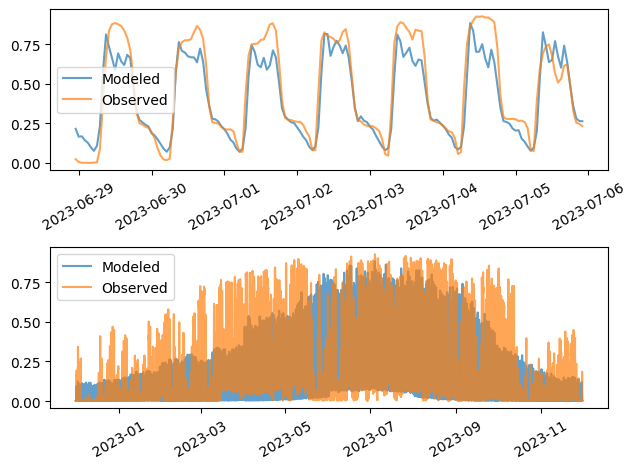
\includegraphics[width=0.7\linewidth]{assets/itransformer-solar-th.png}
    \caption{Weekly and yearly predicted and actual solar TH capacity factor for the iTransformer model}
    \label{fig:itransformer-solar-th}
\end{figure}
In this case, the same ruggedness problem can be seen, which is common to all NN and transformer based models. However, the solar thermal series is not as smooth as the solar photovoltaic so it does not stand as much. It can also be seen how the model accurately models the nightime generation for solar thermal. 
As for the yearly pattern, the model seems to greatly underestimate generation during the winter months and it also assumes a much more uniform generation profile than the real one. 
\subsection{Wind}
The last of the three series is the most different compared to the other two, given the much lower seasonality in wind production and its higher degree of dependence on past cross series. The results obtained for the wind series are the following. Note how in this case both the positive and negative extreme values hold some interest as the lower end of the distribution is no longer zero. In fact, moments of very low wind generation are of special interest given these are the moments when the rest of the energy sources would have to step up.  

\newpage
\begin{table}[ht]
    \footnotesize
    \begin{tabular}[l]{r|c|ccc|cc|}
        \toprule
        \textbf{Wind} &Benchmark&Regression&SARIMAX&VARMAX&SVM&XGBoost \\ 
        \midrule            
        Cramer von Mises&9.483&1783&1814&360.4&434.2&774.6 \\
        KL divergence&0.001479&1.109&1.208&0.1067&0.1318&0.3214 \\
        ACF$_\xi$ distance&0.06016&0.3458&0.3143&0.4598&0.3302&0.6625 \\
        \midrule
        CCMD&0.01117&0.3291&0.1044&0.2151&0.8375&0.3549 \\
        CCF$_\xi^{Solar PV}$ distance&0.01282&0.1621&0.1686&0.05547&0.115&0.4045 \\
        CCF$_\xi^{Solar TH}$ distance&0.01363&0.242&0.2763&0.0691&0.0808&0.525 \\
        \midrule
        CVaR$^+$ distance&-0.02357&0.4225&0.06328&-0.03603&0.02966&-0.5748 \\
        CVaR$^-$ distance&-0.2462&5.582&6.485&3.104&2.912&5.746 \\
        Tail dependence coefficient$^+$&0.04795&0.09132&0.1256&0.1301&0.1119&0.05028 \\
        Tail dependence coefficient$^-$&0.1507&0.1027&0.1553&0.1484&0.05023&0.05003 \\
        Return level distance$^+$&1.362&-0.4957&-0.4707&-0.5817&-0.5813&-1.081 \\
        Return level distance$^-$&-13.51&-7.643&-8.188&-4.958&-3.629&-5.709 \\
        \bottomrule
    \end{tabular}
\end{table}
\begin{table}[ht]
    \footnotesize
    \begin{flushright}
    \begin{tabular}[r]{|ccc|cccc}
        \toprule
        N-BEATS&N-HiTS&TimeMixer&TFT&Informer&FEDFormer&iTransformer  \\
        \midrule            
        381.2&504&553.8&729.6&1283&236&309.9 \\
        0.4356&0.2818&0.2442&0.3298&0.6615&0.1116&0.1838 \\
        0.2918&0.4957&0.2992&0.3452&0.5537&0.3348&0.3312 \\
        \midrule
        0.1959&0.4296&0.05632&0.5398&0.5675&0.5183&0.2093 \\
        0.03014&0.03572&0.04976&0.3294&0.4744&0.03619&0.1731 \\
        0.1954&0.7625&0.06438&0.4002&0.7358&0.03586&0.2802 \\
        \midrule
        -0.5646&-0.504&-0.3975&-0.5549&-0.1147&0.5273&-0.395 \\
        2.788&4.813&3.941&5.036&4.858&0.7204&3.297 \\
        0.09132&0.105&0.08904&0.05479&0.02727&0.02968&0.07534 \\
        0.1119&0.1005&0.09589&0.05251&0.1005&0.04795&0.1872 \\
        -0.8006&-0.9889&-0.8401&-0.9307&-0.4494&0.7511&-0.786 \\
        -2.105&-1.986&-5.443&-6.162&-6.413&-0.6112&-1.679 \\
        \bottomrule
    \end{tabular}
    \end{flushright}
    \caption{Results of the different models for Wind\label{long}}
    \label{table:results-wind}
\end{table}

The rank of each of the models can be seen in \autoref{table:results-rank-wind}. Note how in this case, since both the upper and lower extreme metrics are evaluated, the weight of the extreme value metrics in the total rank will be higher and can skew the percieved overall performance of the models when using this metric.

\newpage
\begin{table}[ht]
    \footnotesize
    \begin{tabular}[l]{r|c|ccc|cc|}
        \toprule
        \textbf{Wind} &Benchmark&Regression&SARIMAX&VARMAX&SVM&XGBoost \\
        \midrule            
        Cramer von Mises&(1)&(12)&(13)&(4)&(6)&(10) \\
        KL divergence&(1)&(12)&(13)&\textbf{(2)}&(4)&(8) \\
        ACF$_\xi$ distance&(1)&(9)&(4)&(10)&(5)&(13) \\
        \midrule
        CCMD&(1)&(7)&(3)&(6)&(13)&(8) \\
        CCF$_\xi^{Solar PV}$ distance&(1)&(8)&(9)&(6)&(7)&(12) \\
        CCF$_\xi^{Solar TH}$ distance&(1)&(7)&(8)&(4)&(5)&(11) \\
        \midrule
        CVaR$^+$ distance&(1)&(8)&(4)&(3)&\textbf{(2)}&(13) \\
        CVaR$^-$ distance&(1)&(11)&(13)&(5)&(4)&(12) \\
        Tail dependence coefficient$^+$&(11)&(6)&(2)&\textbf{(1)}&(3)&(10) \\
        Tail dependence coefficient$^-$&(3)&(6)&(2)&(4)&(11)&(12) \\
        Return level distance$^+$&(13)&(3)&(2)&(5)&(4)&(12) \\
        Return level distance$^-$&(13)&(11)&(12)&(6)&(5)&(8) \\
        \bottomrule
        Total&(48)&(100)&(85)&\textbf{(56)}&(69)&(129) \\
        \bottomrule
    \end{tabular}
\end{table}
\begin{table}[ht]
    \footnotesize
    \begin{flushright}
    \begin{tabular}[r]{|ccc|cccc}
        \toprule
        N-BEATS&N-HiTS&TimeMixer&TFT&Informer&FEDFormer&iTransformer \\
        \midrule            
        (5)&(7)&(8)&(9)&(11)&\textbf{(2)}&(3) \\
        (10)&(7)&(6)&(9)&(11)&(3)&(5) \\
        \textbf{(2)}&(11)&(3)&(8)&(12)&(7)&(6) \\
        \midrule
        (4)&(9)&\textbf{(2)}&(11)&(12)&(10)&(5) \\
        \textbf{(2)}&(3)&(5)&(11)&(13)&(4)&(10) \\
        (6)&(13)&(3)&(10)&(12)&\textbf{(2)}&(9) \\
        \midrule
        (12)&(9)&(7)&(11)&(5)&(10)&(6) \\
        (3)&(8)&(7)&(10)&(9)&\textbf{(2)}&(6) \\
        (6)&(4)&(7)&(9)&(13)&(12)&(8) \\
        (5)&(8)&(9)&(10)&(8)&(13)&\textbf{(1)} \\
        (8)&(11)&(9)&(10)&\textbf{(1)}&(6)&(7) \\
        (4)&(3)&(7)&(9)&(10)&\textbf{(1)}&(2) \\
        \bottomrule
        (66)&(92)&(73)&(117)&(116)&(72)&(68) \\
        \bottomrule
    \end{tabular}
    \end{flushright}
    \caption{Results of the rank of the different models for Wind\label{long}}
    \label{table:results-rank-wind}
\end{table}

At a quick glance it can be seen how the results for the wind series are quite different to those of the other two series. In this case, a different transformer based model -- the FEDFormer -- is the best performer. However, this overall result is highly skewed by the extreme value prediction metric, wehre this model does greatly. In the rest of the categories it also does quite good but not comparatively as much. The iTransformer on the other hand drops quite a few positions in the overall ranking, doing not very badly but not being nearly as dominant, with the general distribution being its best category. The TFT and the Informer are again some of the worst performing models. 

In this case, the VARMAX is surprisingly the best model. It is the first series in which this model outperforms the SARIMAX model, most surely due to the integration component not being significant in this series due to its much higher stationarity. The results of the whole statistical category are however quite surprising, as it would seem by looking at the VARMAX that the simplicity of the model were an advantage, preventing it from capturing spurious patterns more present in the wind series. However, the other two simple models are significantly worse performers. 

Another model with a great improvement in performance is the SVM, for the first time ranking among the top models although not standing out specially in any given category. Again, the XGBoost is the worst performing model.

The N-BEATS and TimeMixer models are again doing very good, with the N-HiTS maintining its drop in performance in this complex series. 

As for the transformers, it would seem like they could maybe benefit from their long run complex pattern capabilities for this series, however as it has already been seen in this series simplicity seems to be the way to go. The iTransformer is agian the best out of all transformer based models, followed by the FEDFormer. This latter model is specially good at modelling the lower tail of the distribution. Although it does significantly worse for the upper tail. 

One final difference for this series is how worse all models are compared to the benchmark relatively to the other two series. No matter what metric one looks at, the gap between the best model and the benchmark is significnatly higher than for the other two series, hinting at the existence of unexploited patterns or modeling criteria that are not being leveraged and that thus do not allow the models to represent the wind series as realistically. 

Finally, regarding the evaluation method itself, it is worth noting how for example all of the models including the benchmark have a very significant negative Return level distance $^-$. What this is showing is that the return level for the lower tail is greately underestimated by all models. If all models including the benchmark show the same bias, it could show that there may be a problem with the data used for evaluation itself, where the lower tail distribution was not representative and thus was underestimated by all models.

\begin{figure}[ht]
    \centering
    \captionsetup{justification=centering}
    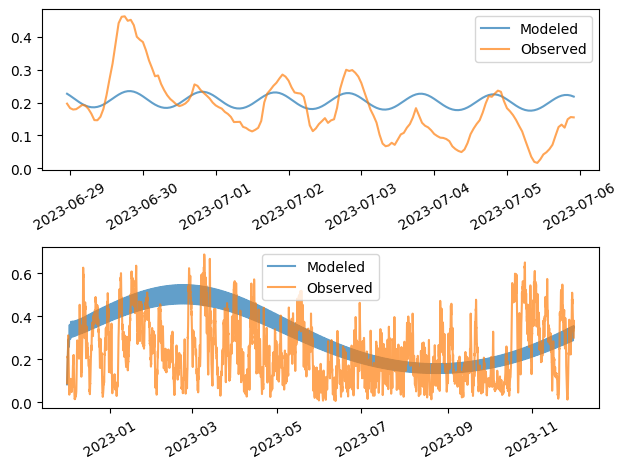
\includegraphics[width=0.7\linewidth]{assets/varmax-wind.png}
    \caption{Weekly and yearly predicted and actual solar TH capacity factor for the iTransformer model}
    \label{fig:varmax-wind}
\end{figure}
The comparison seen in \autoref{fig:varmax-wind} is by far the most discouraging one. It can be seen how the modeled profile distribution has nothing to do with the actual one. The volatility in the modeled data is much lower than the real one, with all of the data being concentrated around a yearly seasonality which only captures very basic yearly and daily profiles -- with the daily ones being present only in the summer, but the model showing them for the whole year. 

It is not very promising that this is the best model that could be found, although using other models not as constrained by the seasonality and simplicity of the VARMAX does not shed much improvement. 

\textcolor{red}{ADD NBEATS PLOT?}

This does shed some light on some necessary changes for future works. It is clear that the wind capacity factor has a really prominent random component and a low signal to noise ratio. The loss functions that have been used, which are mainly MAE and SE as they are the standard for these type of tasks, make the model extremely risk averse in their predictions and when they cannot accurately predict the wind values they end up predicting a kind of mean. For more realistic modeling of wind data it seems like different loss functions that don't penalize point errors that much need to be used. 

\subsection{Custom loss function}
After having analyzed the results for all models in the three capacity factor series, it is now time to analyze the results regarding the hypothesis of the custom loss function. That is, can the behaviour of the model be steered through a custom loss function -- in this case the SERA loss -- to better predict extreme values? As explained in the \nameref{s:loss-function} section, an XGBoost model has been trained using this loss function with the same hyperparameters as the base XGBoost model. In fact, two such models have been implemented, one focusing on the upper tail extreme values and one focusing on the lower tail extreme values. The relevance function in both cases has been to give a relevance of 1 to the top or bottom 10\%, a relevance of 0 to the opposite 10\% and the rest of the distribution is given a relevance based on the spline interpolation. 

Note that the modeling has been done using the custom loss only for the wind modeling, given this is the series where there is a highest practical interest to accurately predict extreme events. The results are as follows. 

\newpage
\begin{table}[ht]
    \centering
    \footnotesize
    \begin{tabular}[r]{r|c|cc}
        \toprule
        \textbf{Wind}&XGBoost&XGBoost$^-$&XGBoost$^+$ \\
        \midrule            
        Cramer von Mises&774.6&1332&1978 \\
        KL divergence&0.3214&0.6029&1.678 \\
        ACF$_\xi$ distance&0.6625&0.6622&0.2574 \\
        \midrule
        CCMD&0.3549&0.3584&0.4519 \\
        CCF$_\xi^{Solar PV}$ distance&0.4045&0.3901&0.3306 \\
        CCF$_\xi^{Solar TH}$ distance&0.525&0.5031&0.4071 \\
        \midrule
        CVaR$^+$ distance&-0.5748&-0.4043&-0.235 \\
        CVaR$^-$ distance&5.746&8.46&11.03 \\
        Tail dependence coefficient$^+$&0.05028&0.05008&0.05974 \\
        Tail dependence coefficient$^-$&0.05003&0.04982&0.01963 \\
        Return level distance$^+$&-1.081&-1.206&-0.81 \\
        Return level distance$^-$&-5.709&-6.974&-8.092 \\
        \bottomrule
    \end{tabular}
    \caption{Results of the XGBoost models with SERA loss functions for Wind\label{long}}
    \label{table:results-custom-loss}
\end{table}

Even though these results are much easier to read and interpret than the ones where all of the models are included, the rank will still be provided in order to help interpret the results as much as possible. 

\begin{table}[ht]
    \centering
    \footnotesize
    \begin{tabular}[r]{r|c|cc}
        \toprule
        \textbf{Wind}&XGBoost&XGBoost$^-$&XGBoost$^+$ \\
        \midrule            
        Cramer von Mises&\textbf{(1)}&(2)&(3) \\
        KL divergence&\textbf{(1)}&(2)&(3) \\
        ACF$_\xi$ distance&(3)&(2)&\textbf{(1)} \\
        \midrule
        CCMD&\textbf{(1)}&(2)&(3) \\
        CCF$_\xi^{Solar PV}$ distance&(3)&(2)&\textbf{(1)} \\
        CCF$_\xi^{Solar TH}$ distance&(3)&(2)&\textbf{(1)} \\
        \midrule
        CVaR$^+$ distance&(3)&(2)&\textbf{(1)} \\
        CVaR$^-$ distance&\textbf{(1)}&(2)&(3) \\
        Tail dependence coefficient$^+$&(2)&(3)&\textbf{(1)} \\
        Tail dependence coefficient$^-$&\textbf{(1)}&(2)&(3) \\
        Return level distance$^+$&(2)&(3)&\textbf{(1)} \\
        Return level distance$^-$&\textbf{(1)}&(2)&(3) \\
        \bottomrule
        Total&\textbf{(22)}&(26)&(24) \\
        \bottomrule
    \end{tabular}
    \caption{Results of the XGBoost models' rank with SERA loss functions for Wind\label{long}}
    \label{table:results-rank-custom-loss}
\end{table}

The first insight that can be obtained from these results is that, unsurprisingly, the unbiased XGBoost model seems to be the one best representing the general distribution of the series. This is to be expected as the other two models will probably have introduced some bias in order to better fit extreme values. However, what is surprising is how the upper tail focused model performs better in all metrics regarding temporal consistency both for the series with itself and with the other two series. This probably means that higher wind capacity factor values are more realted to previous wind and solar values than the lower ones. 

Interestingly, this holds not only for the self temporal correlation but also for the cross temporal correlation, with this model being the also the best one regarding the correlation of the wind values with lagged values of the other two series. 

Regarding extreme values, which is actually the whole purpose of introducing the custom loss function, a couple interesting observations can be made. Introducing the SERA loss seems to correctly steer the model into correctly modeling the upper tail of the wind capacity factor. However, this result cannot be replicated for the lower tail and the unbiased model is actually the one with the best performance in the lower extreme values. 
\newpage
\section{Conclusion}
Outline with conribution, summary of findings, limitations, future work

\newpage
\begin{appendices}
\section{Code implementation}
\label{sec:code}
The code used in this work has been made publicly accessible. That is, the implementation of the different models, but also all the code use to train and evaluate them, the preliminary study of the datasets, etc. Even the latex version of this written document has been made accessible. All that code can be accessed via GitHub at \href{https://github.com/fcelya/solar-wind-generation}{https://github.com/fcelya/solar-wind-generation}. The only elements that have not been made accessible are the datasets used to run the strategy and to estimate the factor parameters. They could not be uploaded due to GitHub's limitations, and enough information has been given in \autoref{sec:data-description} for anyone to be able to recreate those datasets. \\ The hope is that by making this code easily accessible, more people will be tempted to explore it, play with it, tackle the problem of long term solar and wind energy modeling and the ideas presented in this work can be further explored by the community at large.

Some of the code used to generate the results in this work are not present in the mentioned repository. Due to the compute needed to train the neural network and transformer based models, these models have been trained in Google Colab and Kaggle Notebook environments, leveraging their freely accessible GPU and TPU infraestructure. For many of these neural network and transformer based models, they have been implemented through the open source library NeuralForecast created by Nixtla. For more information refer to \cite{olivares2022library_neuralforecast}.
\newpage
\end{appendices}

\printbibliography[heading=bibintoc]
\end{document}
